
\subsection{Plotted Limits}
%%%%%%%%%%%%%%%%%%%%%%%%%%%%%%

\subsubsection{Zero-Jet Cut-Based}
\begin{figure}[!htbp]
\centering
\subfigure[]{
\centering
\label{subfig:lp_0j_sf_cut}
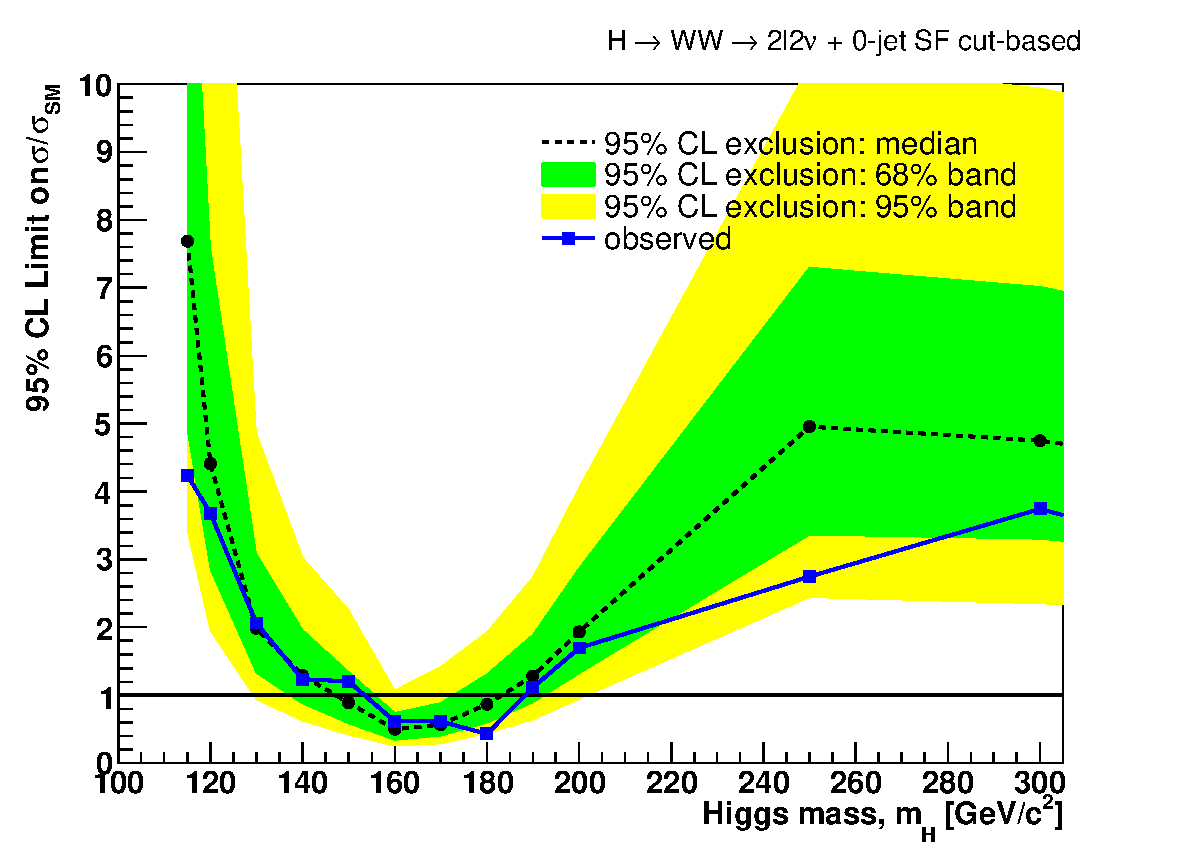
\includegraphics[width=0.48\textwidth]{lp_figures/limits_0j_sf_cut.pdf}}
\subfigure[]{
\centering
\label{subfig:lp_0j_of_cut}
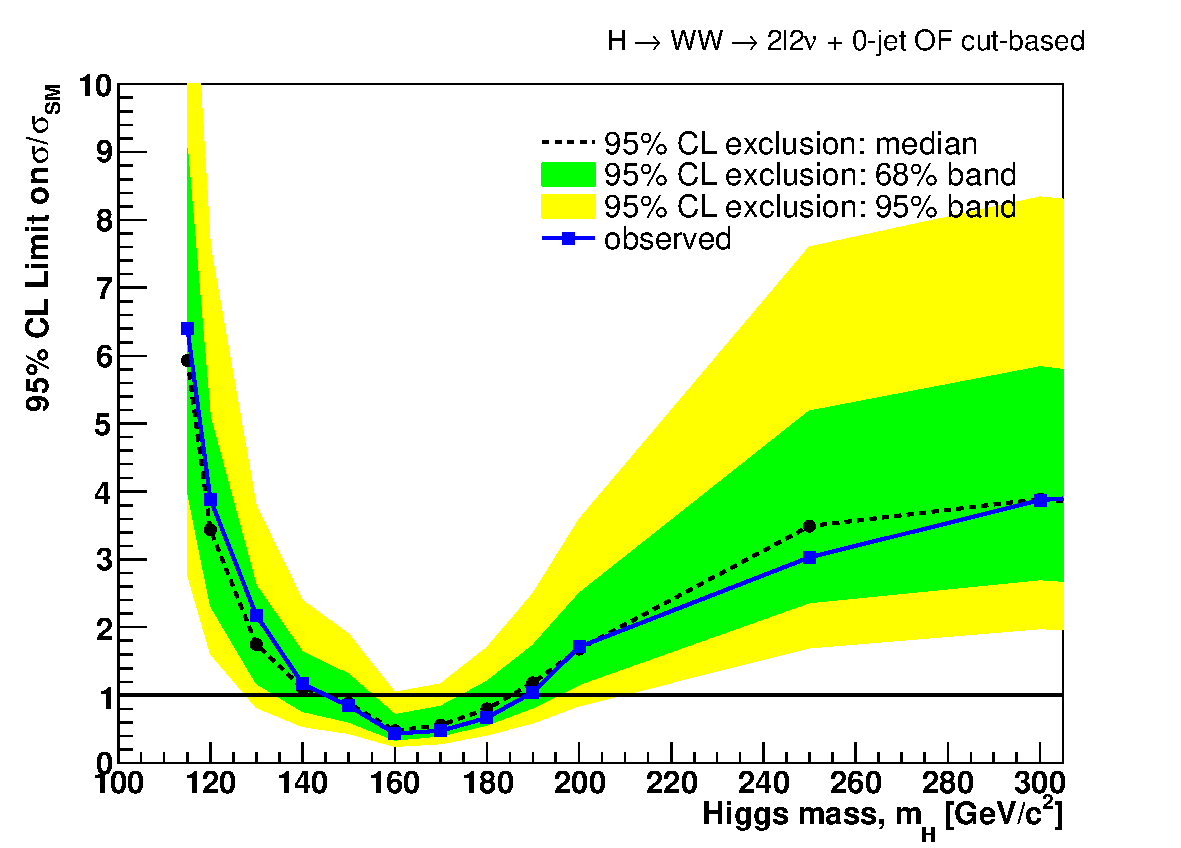
\includegraphics[width=0.48\textwidth]{lp_figures/limits_0j_of_cut.pdf}}
\subfigure[]{
\centering
\label{subfig:eps_0j_sf_cut}
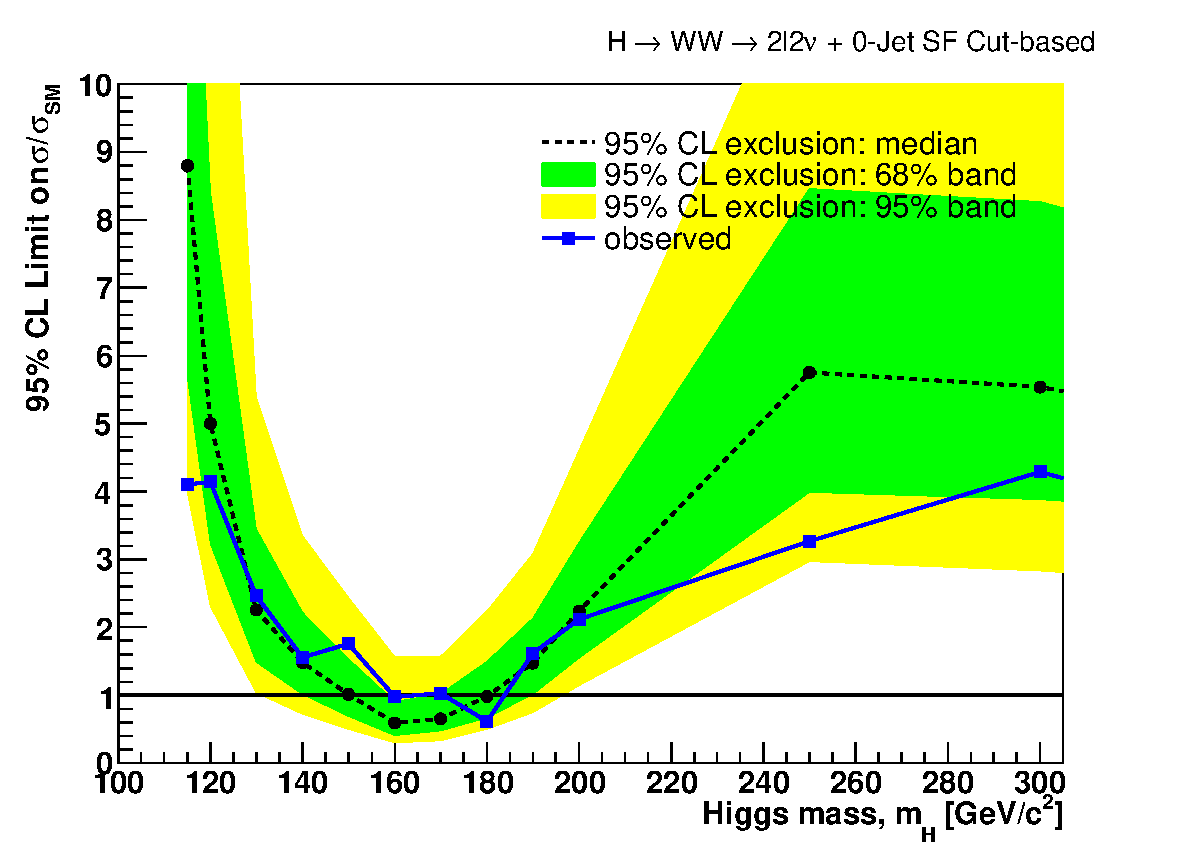
\includegraphics[width=0.48\textwidth]{lp_figures/limits_0j_sf_cut_ana_v6_1500pb_LP_EPS.pdf}}
\subfigure[]{
\centering
\label{subfig:eps_0j_of_cut}
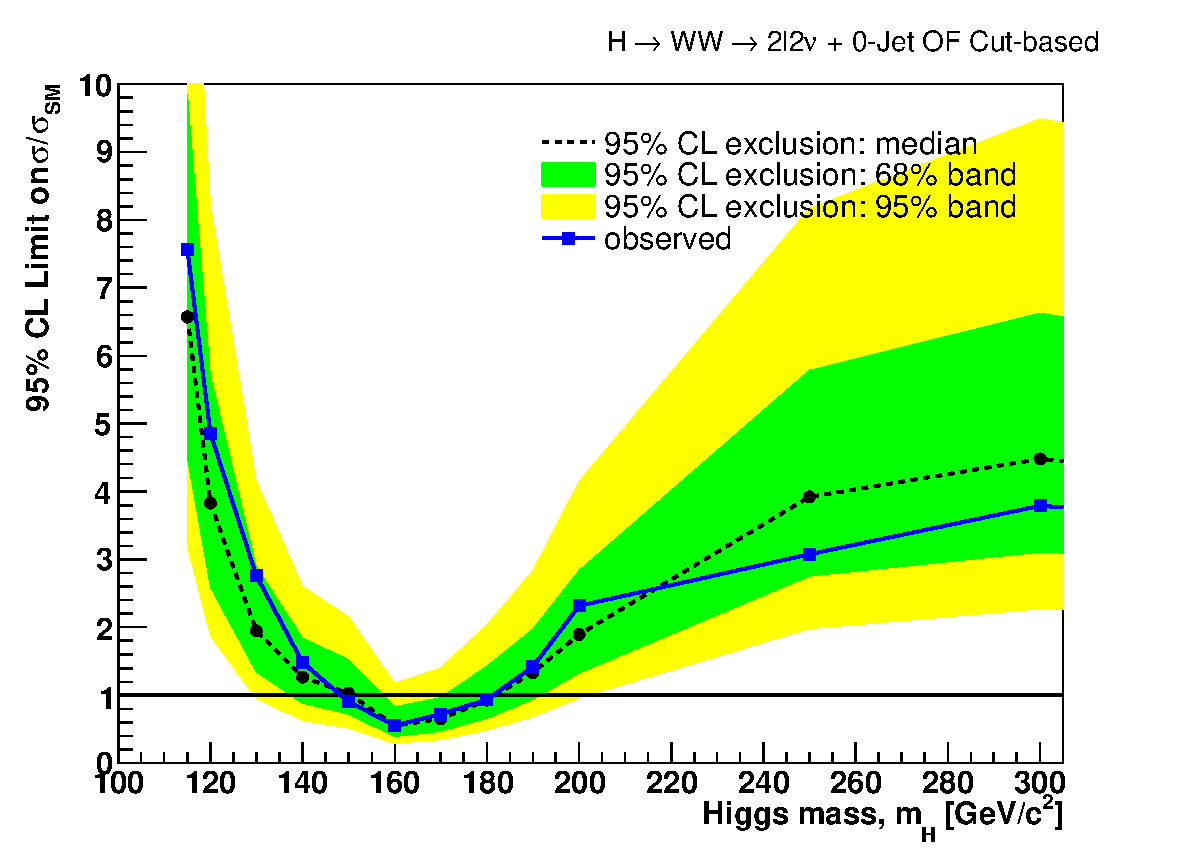
\includegraphics[width=0.48\textwidth]{lp_figures/limits_0j_of_cut_ana_v6_1500pb_LP_EPS.pdf}}
\subfigure[]{
\centering
\label{subfig:post_0j_sf_cut}
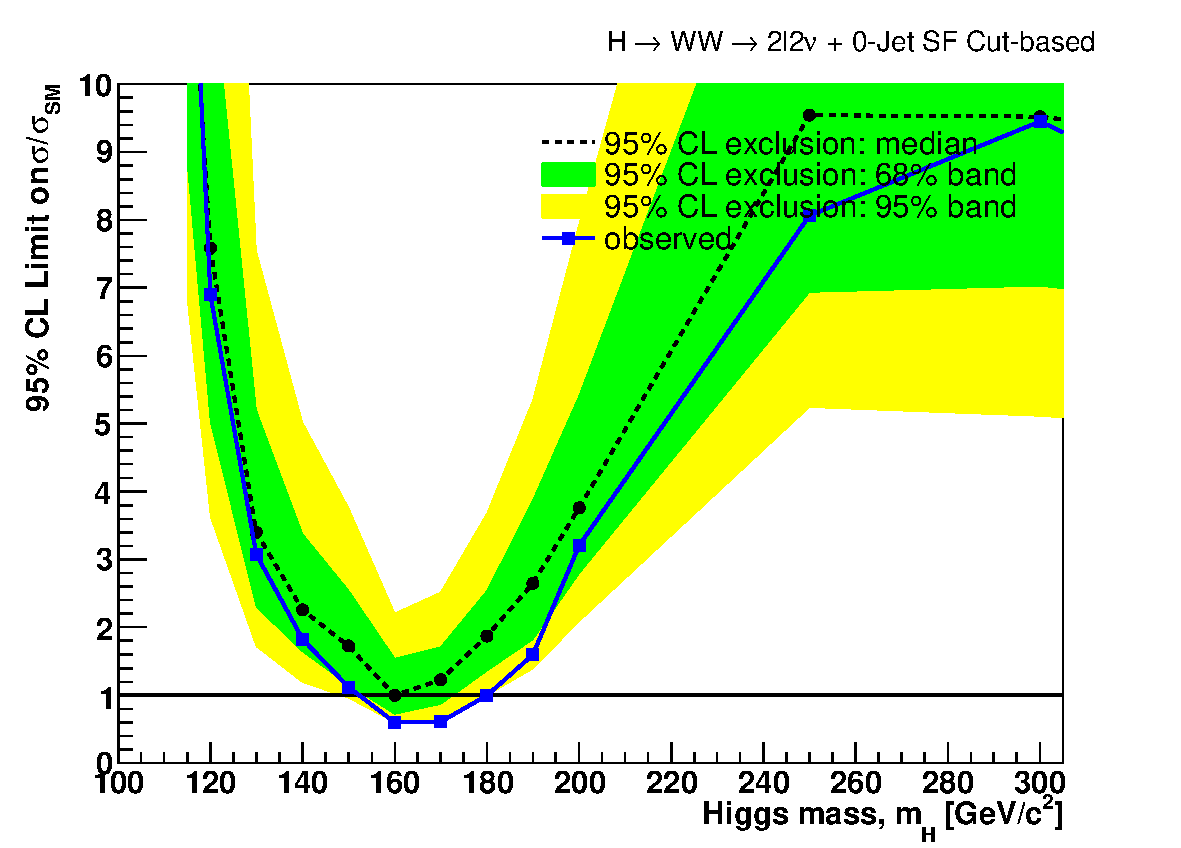
\includegraphics[width=0.48\textwidth]{lp_figures/limits_0j_sf_cut_ana_v6_1500pb_LP_POSTEPS.pdf}}
\subfigure[]{
\centering
\label{subfig:post_0j_of_cut}
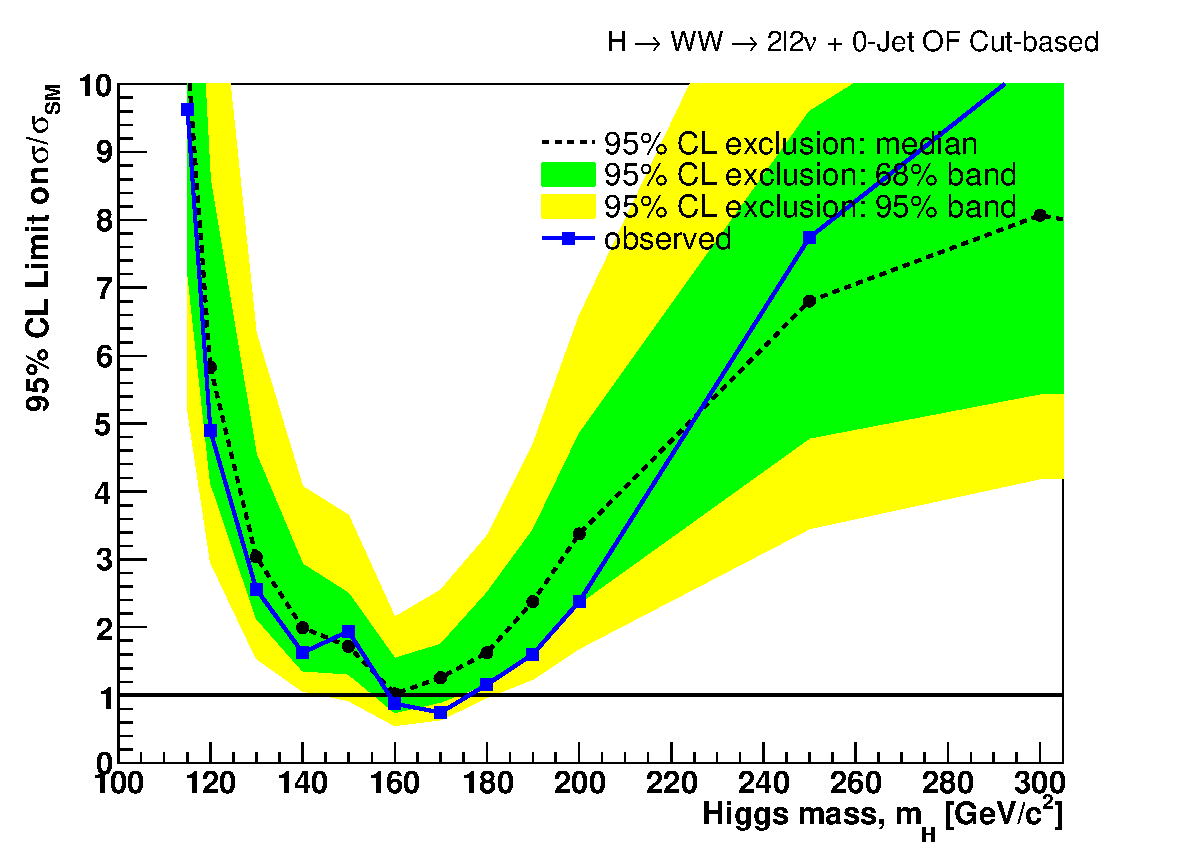
\includegraphics[width=0.48\textwidth]{lp_figures/limits_0j_of_cut_ana_v6_1500pb_LP_POSTEPS.pdf}}
\caption{Cut-based analysis upper limits at 95\% C.L. using LP, EPS and post-EPS datasets for 0-jet events.
\subref{subfig:lp_0j_sf_cut}: LP same-flavor; \subref{subfig:lp_0j_of_cut}: LP opposite-flavor;
\subref{subfig:eps_0j_sf_cut}: EPS same-flavor; \subref{subfig:eps_0j_of_cut}: EPS opposite-flavor;
\subref{subfig:post_0j_sf_cut}: post-EPS same-flavor; \subref{subfig:post_0j_of_cut}: post-EPS opposite-flavor;
}
\label{fig:limits_0j_cut}
\end{figure}

\clearpage
\subsubsection{Zero-Jet MVA-Based}
\begin{figure}[!htbp]
\centering
\subfigure[]{
\centering
\label{subfig:lp_0j_sf_shape}
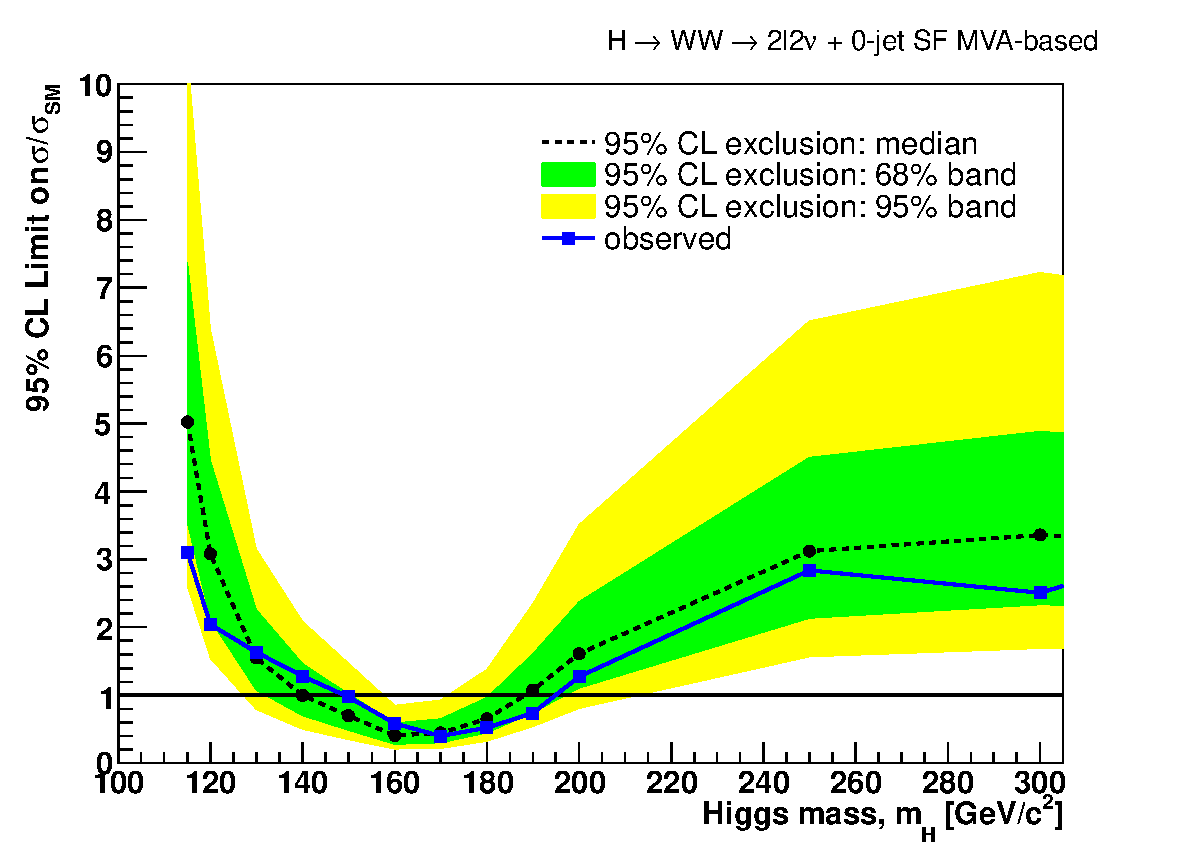
\includegraphics[width=0.48\textwidth]{lp_figures/limits_0j_sf_shape.pdf}}
\subfigure[]{
\centering
\label{subfig:lp_0j_of_shape}
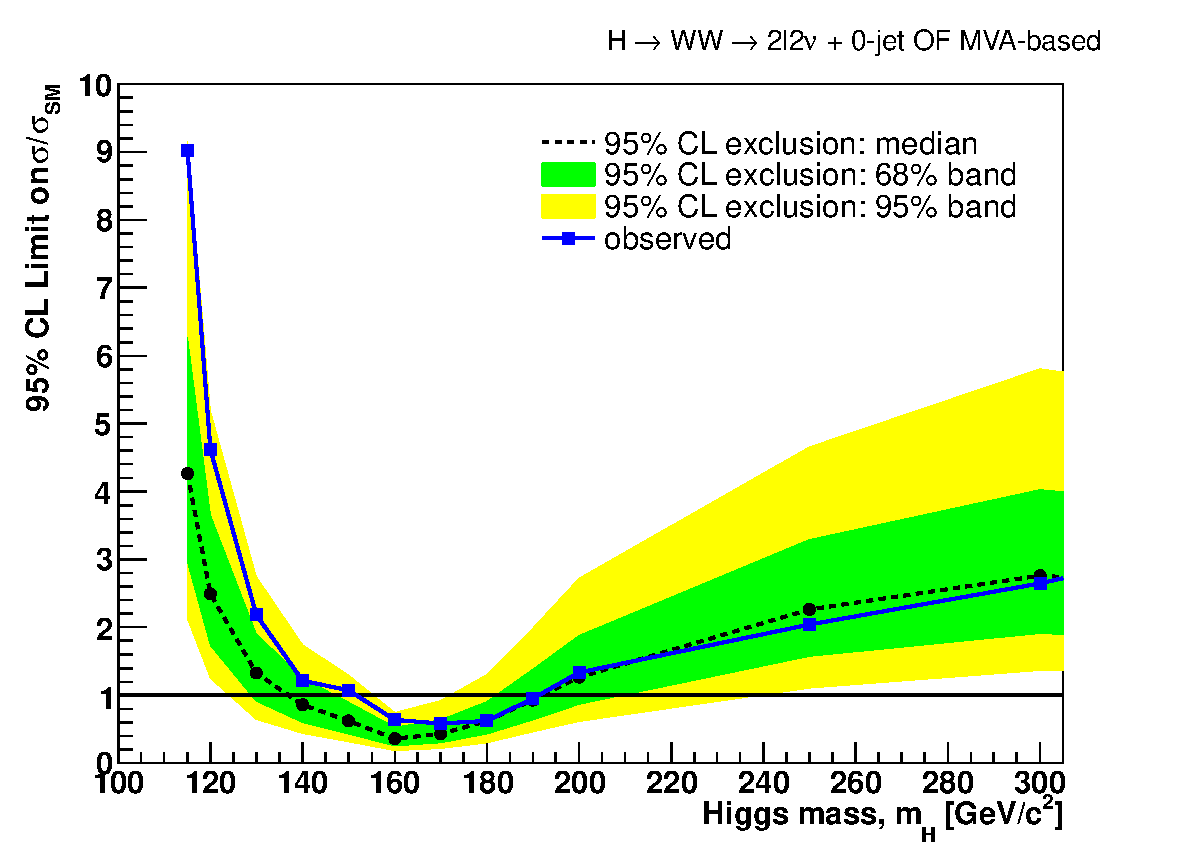
\includegraphics[width=0.48\textwidth]{lp_figures/limits_0j_of_shape.pdf}}
\subfigure[]{
\centering
\label{subfig:eps_0j_sf_shape}
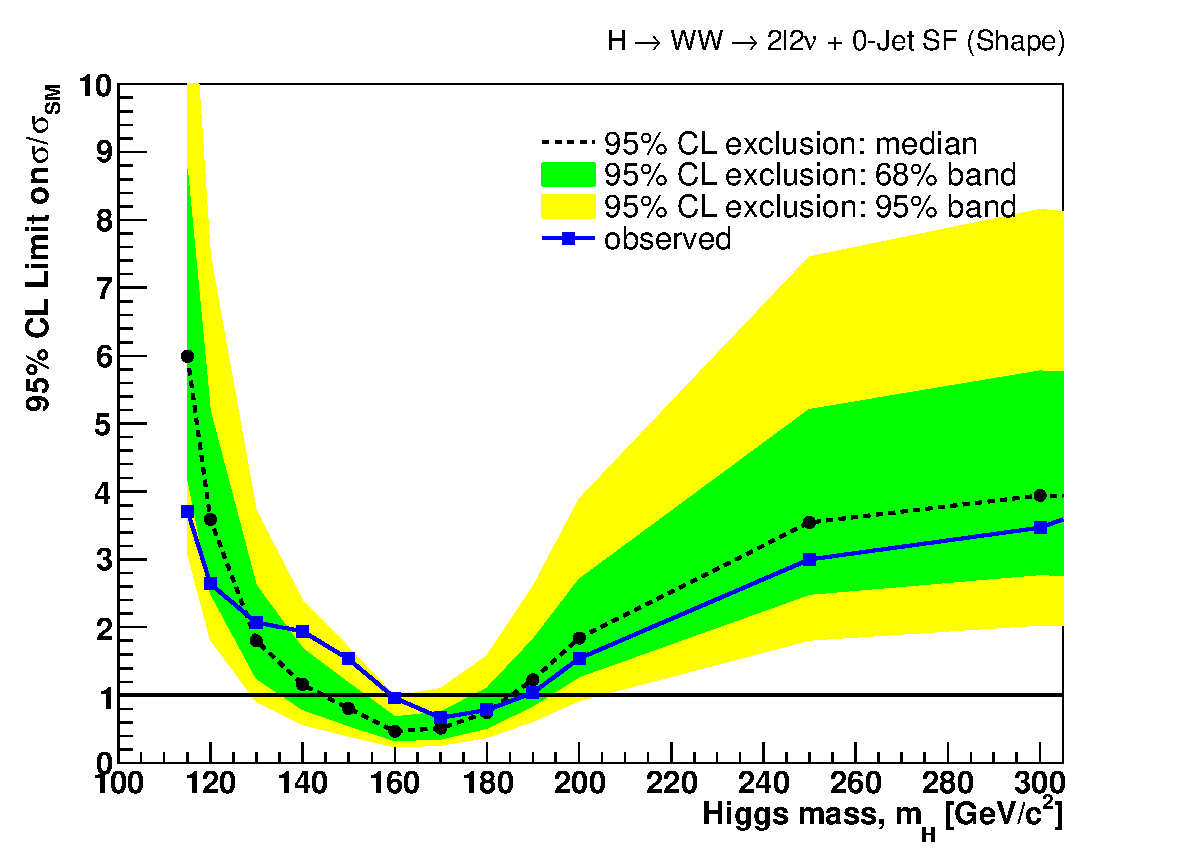
\includegraphics[width=0.48\textwidth]{lp_figures/limits_0j_sf_shape_ana_v6_1500pb_LP_EPS.pdf}}
\subfigure[]{
\centering
\label{subfig:eps_0j_of_shape}
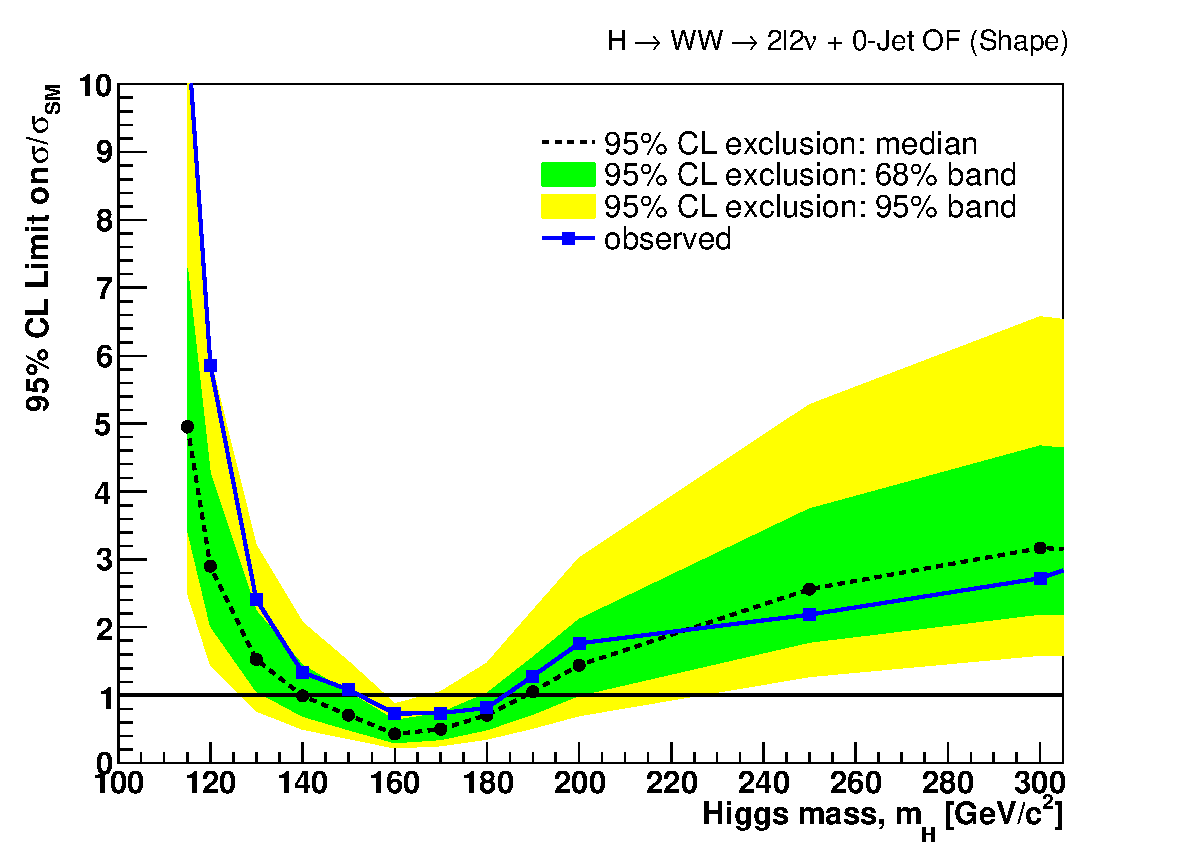
\includegraphics[width=0.48\textwidth]{lp_figures/limits_0j_of_shape_ana_v6_1500pb_LP_EPS.pdf}}
\subfigure[]{
\centering
\label{subfig:post_0j_sf_shape}
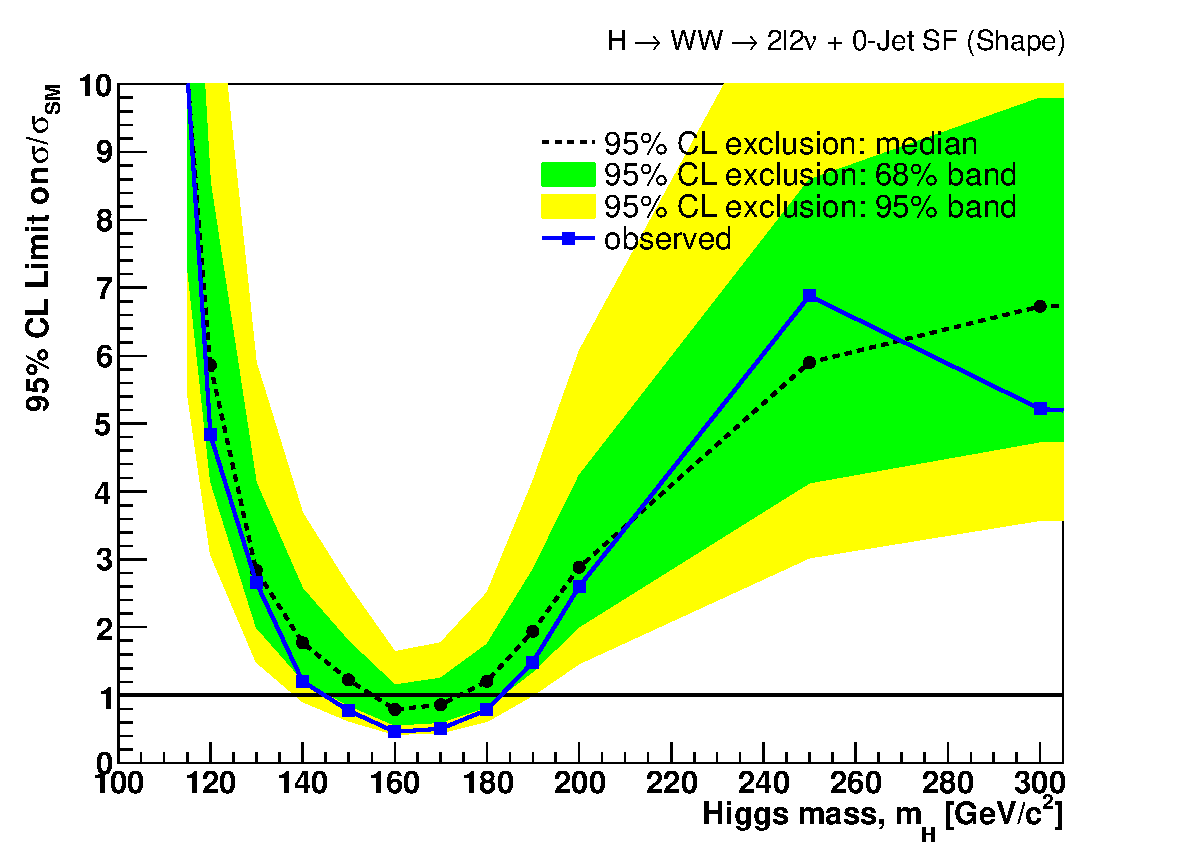
\includegraphics[width=0.48\textwidth]{lp_figures/limits_0j_sf_shape_ana_v6_1500pb_LP_POSTEPS.pdf}}
\subfigure[]{
\centering
\label{subfig:post_0j_of_shape}
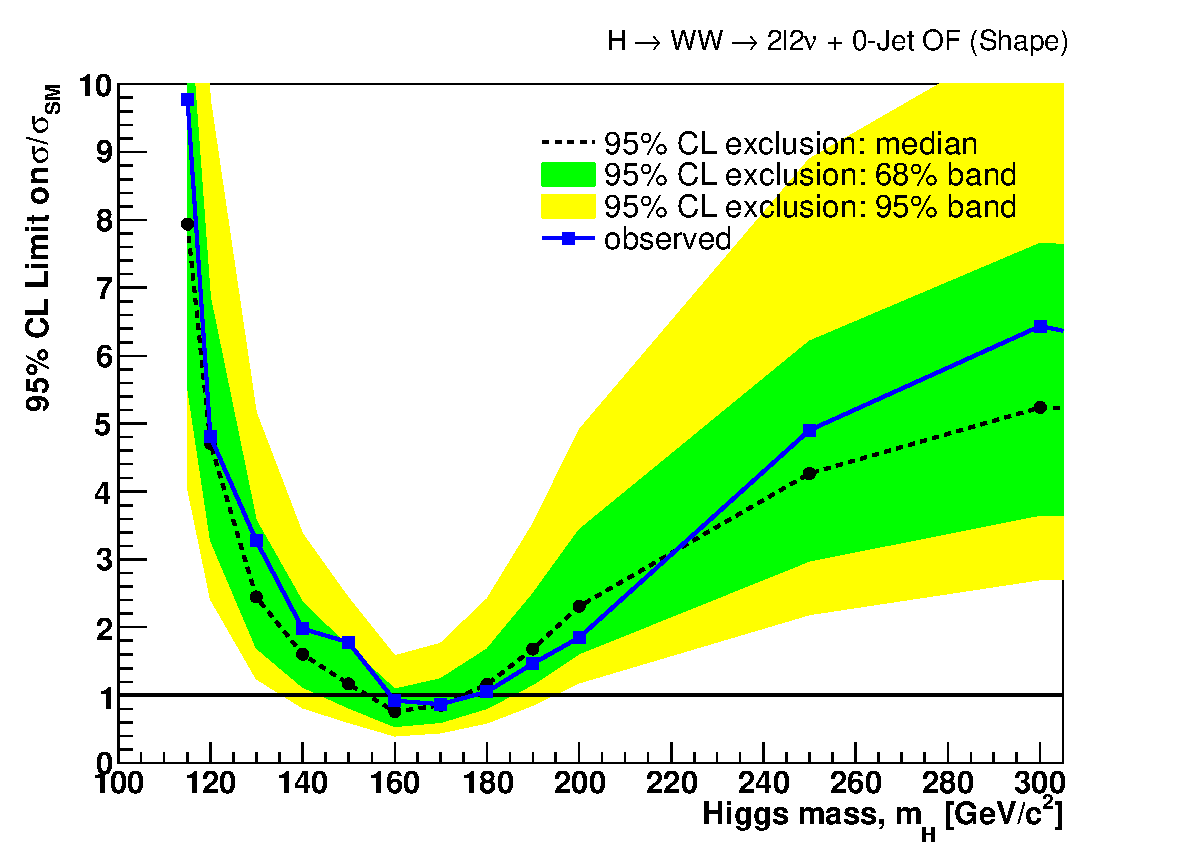
\includegraphics[width=0.48\textwidth]{lp_figures/limits_0j_of_shape_ana_v6_1500pb_LP_POSTEPS.pdf}}
\caption{Multivariate-based analysis upper limits at 95\% C.L. using LP, EPS and post-EPS datasets for 0-jet events.
\subref{subfig:lp_0j_sf_shape}: LP same-flavor; \subref{subfig:lp_0j_of_shape}: LP opposite-flavor;
\subref{subfig:eps_0j_sf_shape}: EPS same-flavor; \subref{subfig:eps_0j_of_shape}: EPS opposite-flavor;
\subref{subfig:post_0j_sf_shape}: post-EPS same-flavor; \subref{subfig:post_0j_of_shape}: post-EPS opposite-flavor;
}
\label{fig:limits_0j_shape}
\end{figure}

\clearpage
\subsubsection{One-Jet Cut-Based}
\begin{figure}[!htbp]
\centering
\subfigure[]{
\centering
\label{subfig:lp_1j_sf_cut}
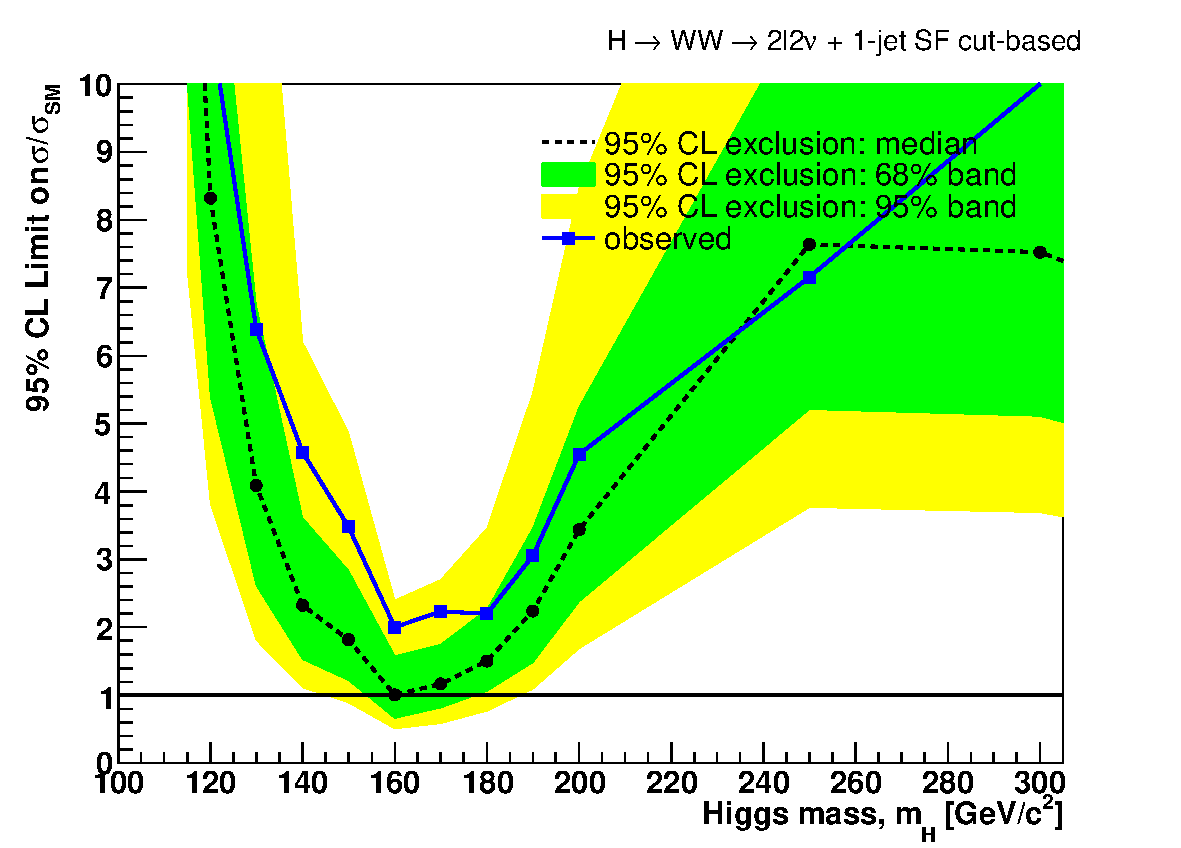
\includegraphics[width=0.48\textwidth]{lp_figures/limits_1j_sf_cut.pdf}}
\subfigure[]{
\centering
\label{subfig:lp_1j_of_cut}
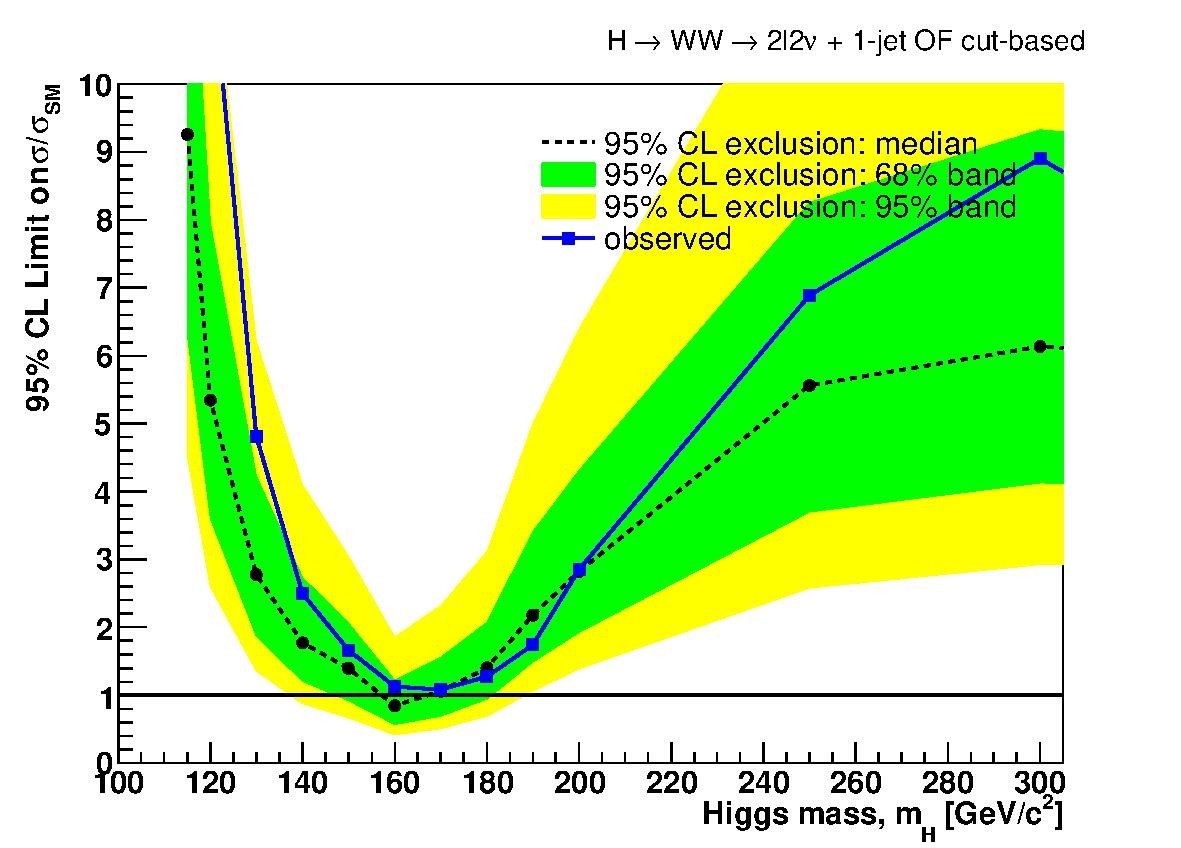
\includegraphics[width=0.48\textwidth]{lp_figures/limits_1j_of_cut.pdf}}
\subfigure[]{
\centering
\label{subfig:eps_1j_sf_cut}
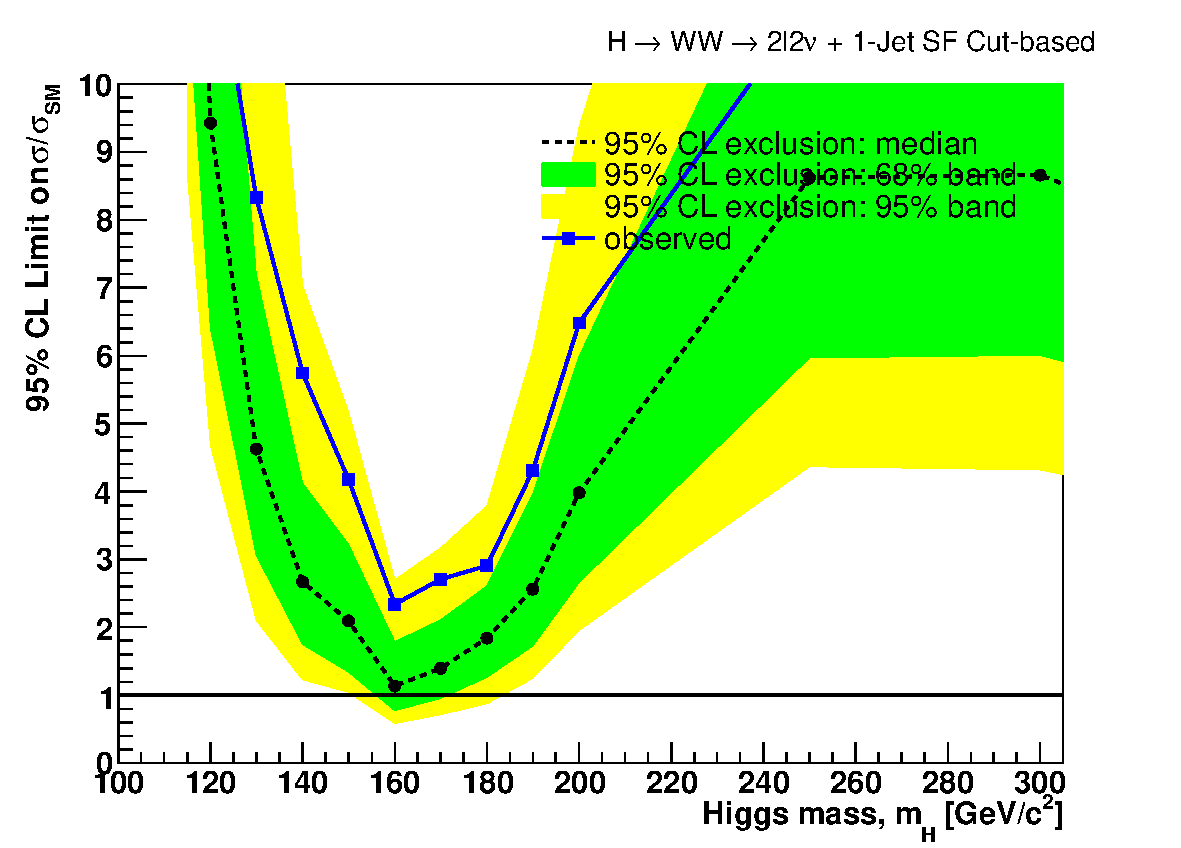
\includegraphics[width=0.48\textwidth]{lp_figures/limits_1j_sf_cut_ana_v6_1500pb_LP_EPS.pdf}}
\subfigure[]{
\centering
\label{subfig:eps_1j_of_cut}
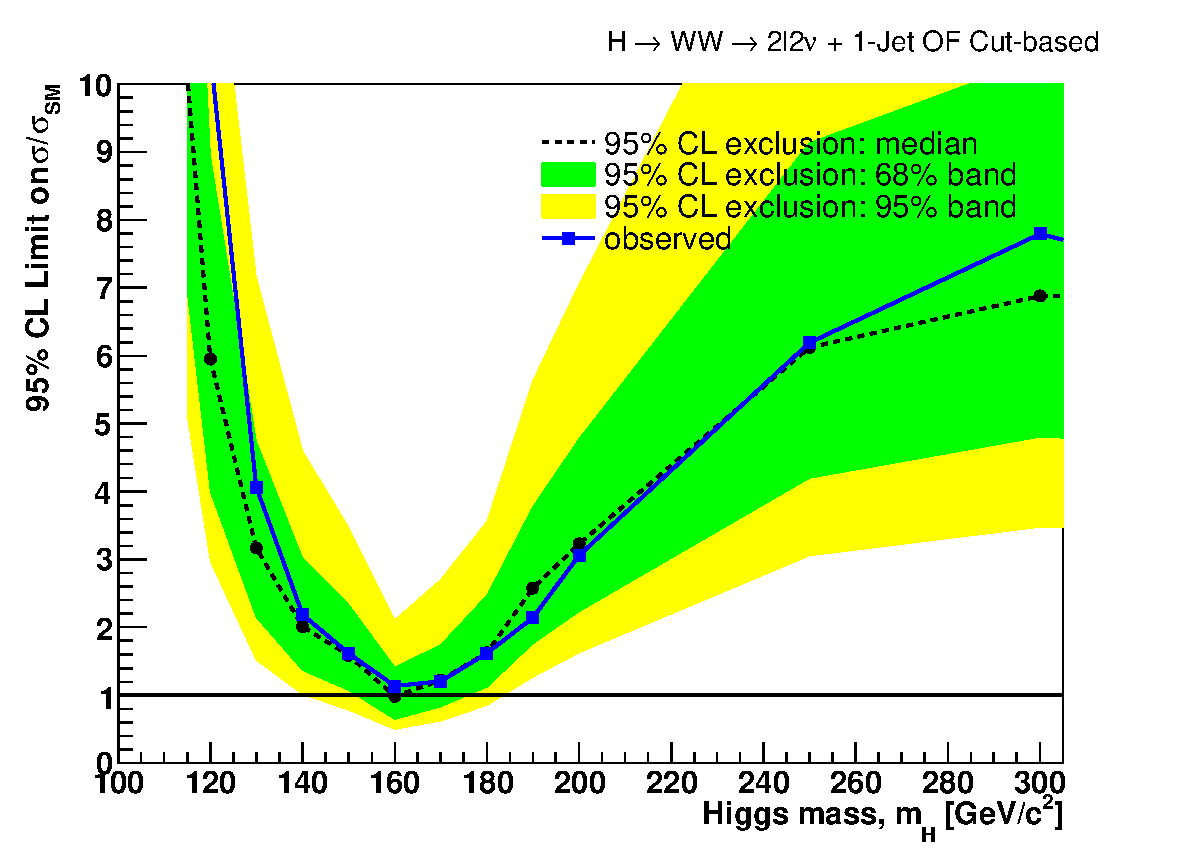
\includegraphics[width=0.48\textwidth]{lp_figures/limits_1j_of_cut_ana_v6_1500pb_LP_EPS.pdf}}
\subfigure[]{
\centering
\label{subfig:post_1j_sf_cut}
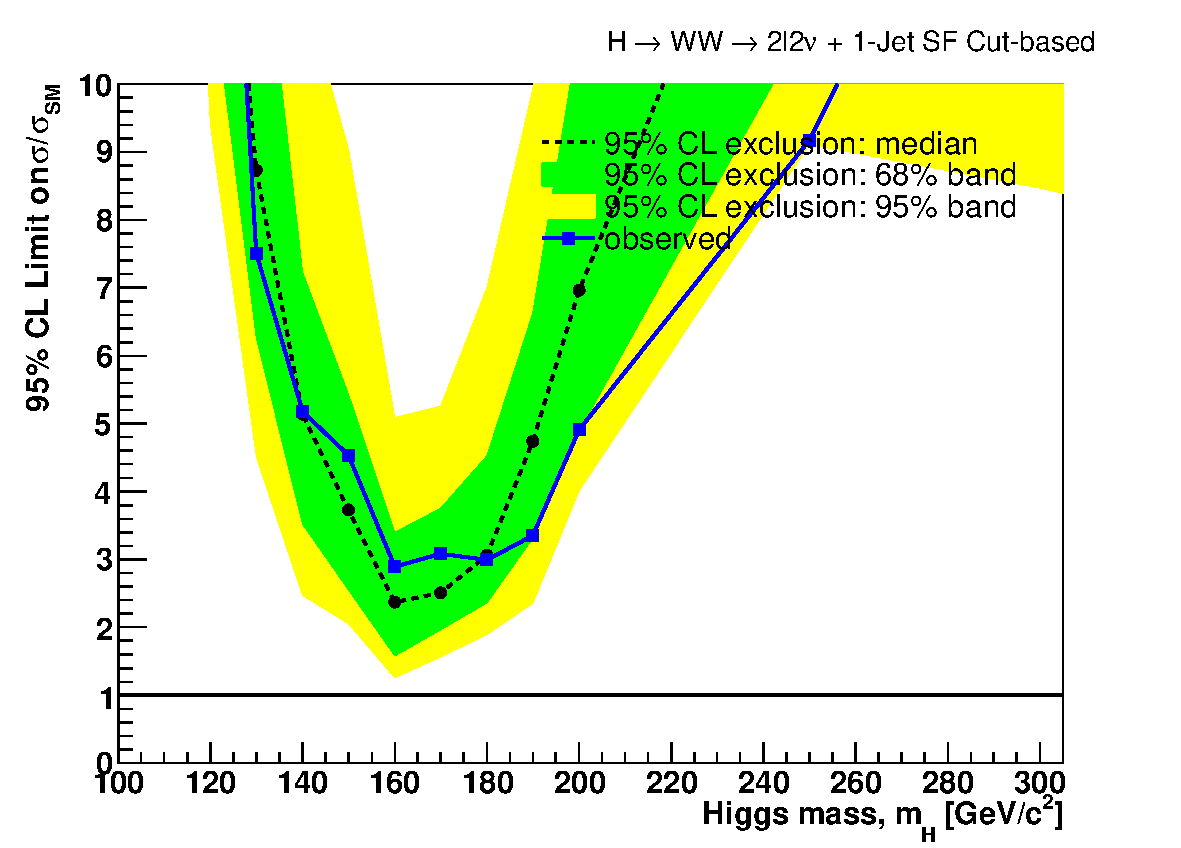
\includegraphics[width=0.48\textwidth]{lp_figures/limits_1j_sf_cut_ana_v6_1500pb_LP_POSTEPS.pdf}}
\subfigure[]{
\centering
\label{subfig:post_1j_of_cut}
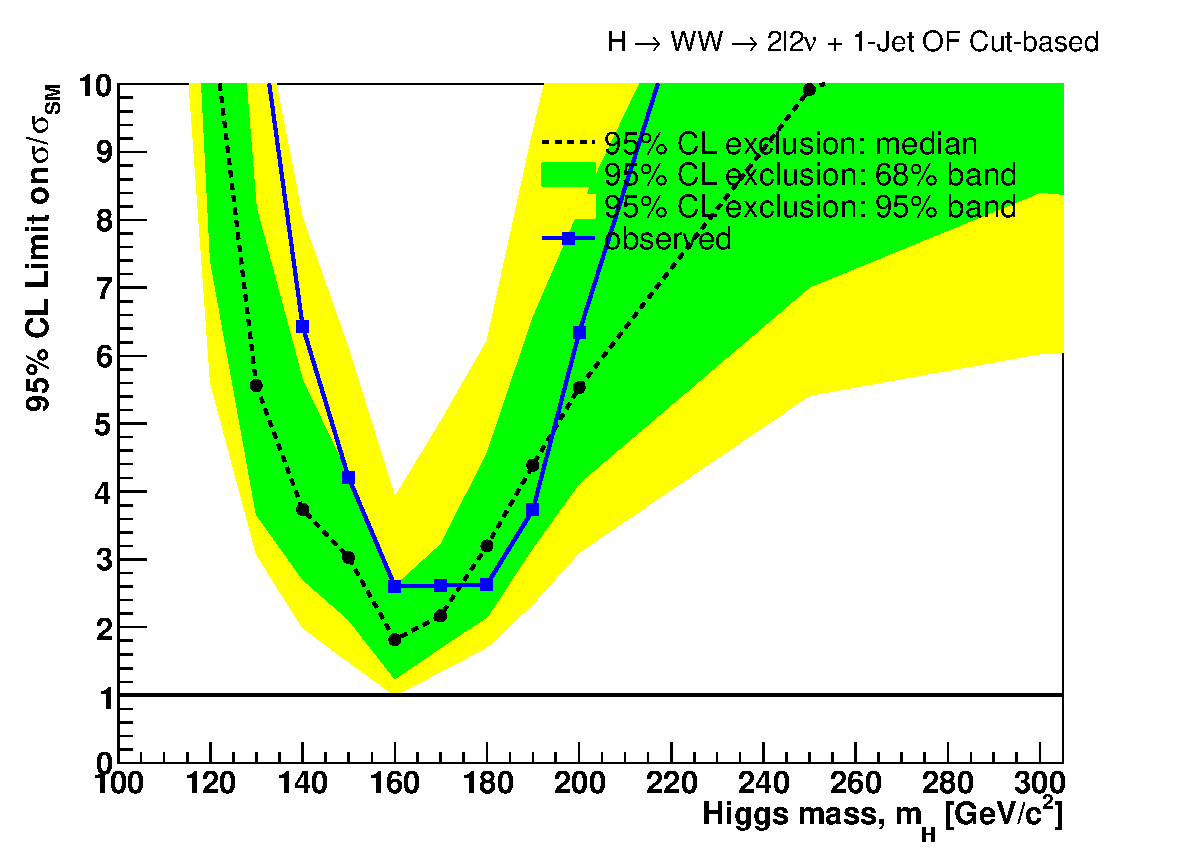
\includegraphics[width=0.48\textwidth]{lp_figures/limits_1j_of_cut_ana_v6_1500pb_LP_POSTEPS.pdf}}
\caption{Cut-based analysis upper limits at 95\% C.L. using LP, EPS and post-EPS datasets for 1-jet events.
\subref{subfig:lp_1j_sf_cut}: LP same-flavor; \subref{subfig:lp_1j_of_cut}: LP opposite-flavor;
\subref{subfig:eps_1j_sf_cut}: EPS same-flavor; \subref{subfig:eps_1j_of_cut}: EPS opposite-flavor;
\subref{subfig:post_1j_sf_cut}: post-EPS same-flavor; \subref{subfig:post_1j_of_cut}: post-EPS opposite-flavor;
}
\label{fig:limits_1j_cut}
\end{figure}

\clearpage
\subsubsection{One-Jet MVA-Based}
\begin{figure}[!htbp]
\centering
\subfigure[]{
\centering
\label{subfig:lp_1j_sf_shape}
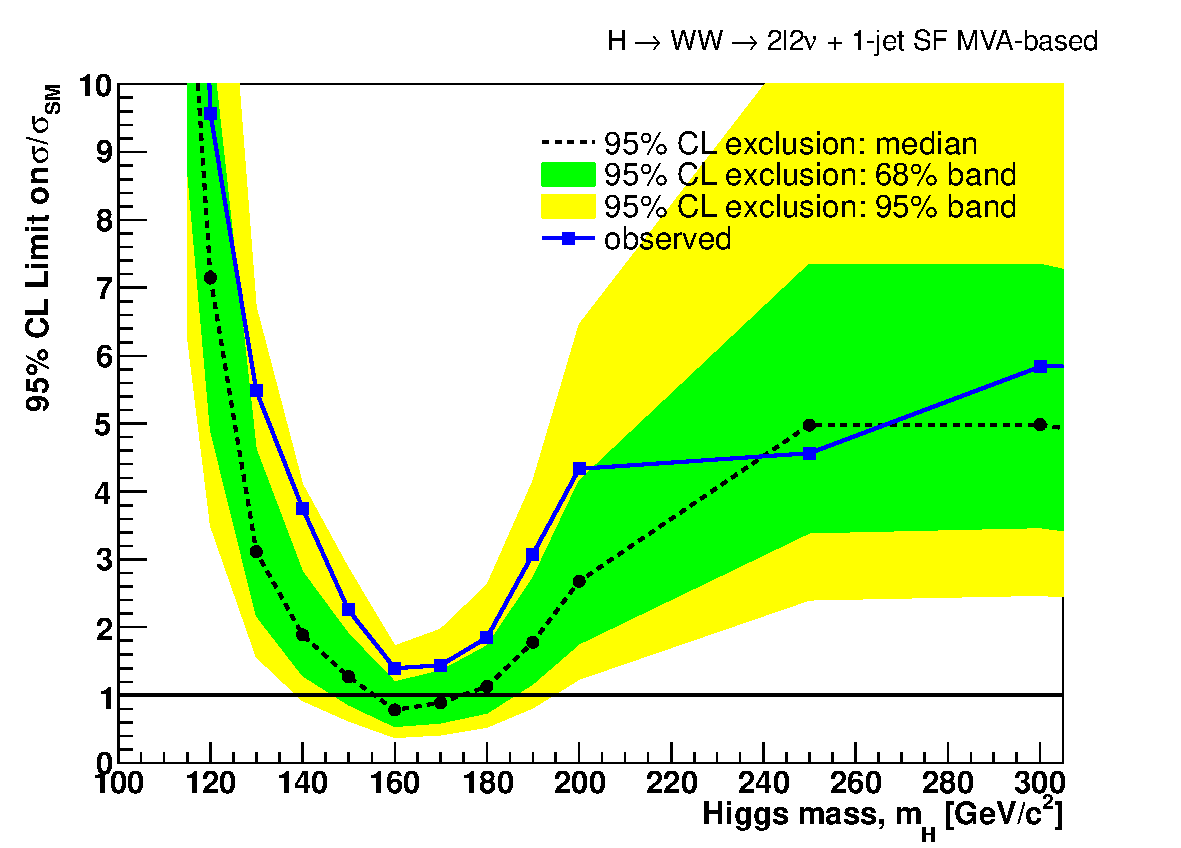
\includegraphics[width=0.48\textwidth]{lp_figures/limits_1j_sf_shape.pdf}}
\subfigure[]{
\centering
\label{subfig:lp_1j_of_shape}
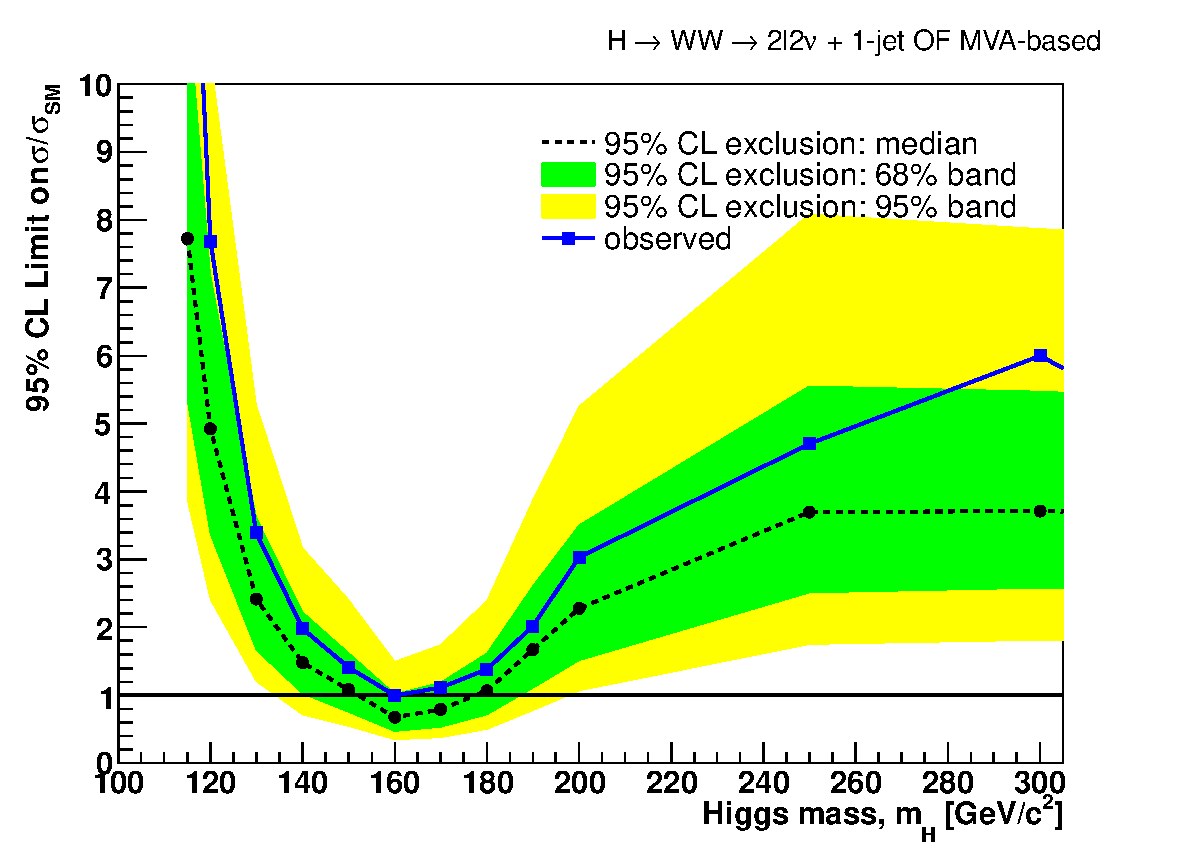
\includegraphics[width=0.48\textwidth]{lp_figures/limits_1j_of_shape.pdf}}
\subfigure[]{
\centering
\label{subfig:eps_1j_sf_shape}
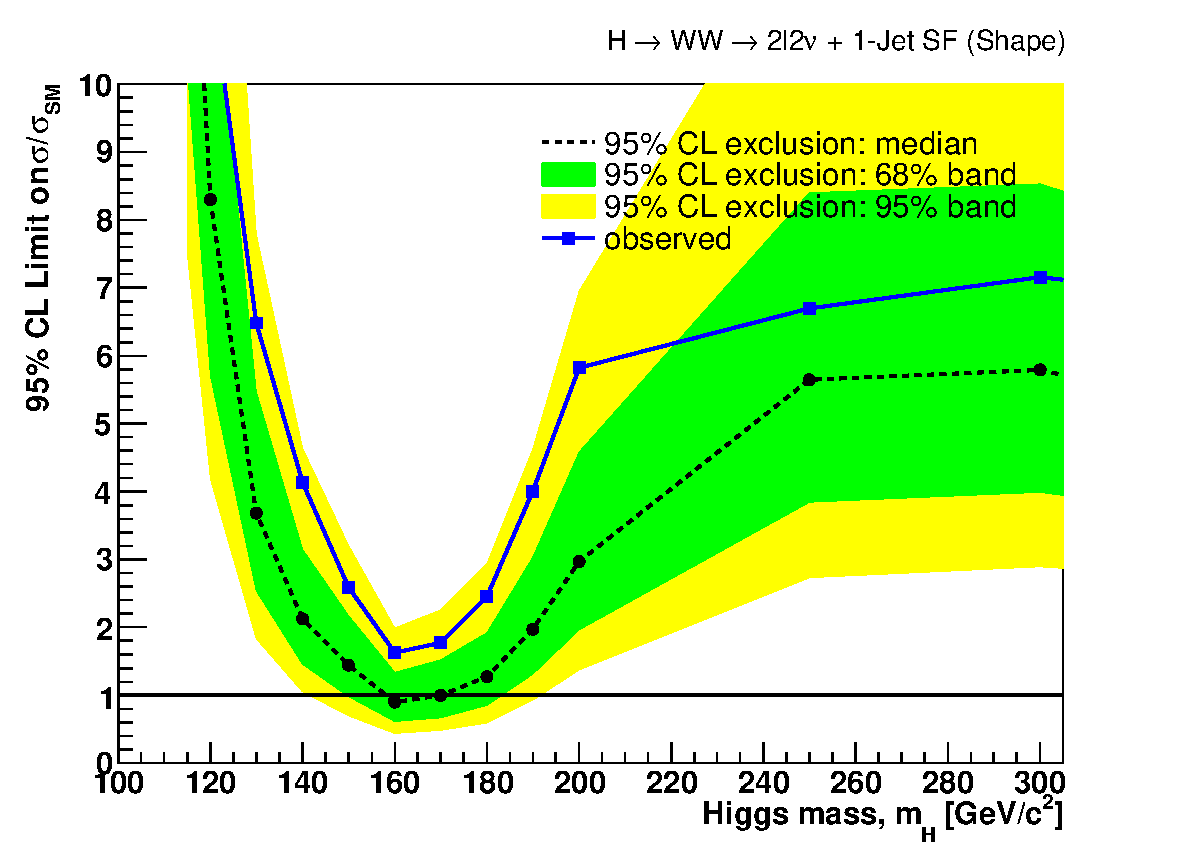
\includegraphics[width=0.48\textwidth]{lp_figures/limits_1j_sf_shape_ana_v6_1500pb_LP_EPS.pdf}}
\subfigure[]{
\centering
\label{subfig:eps_1j_of_shape}
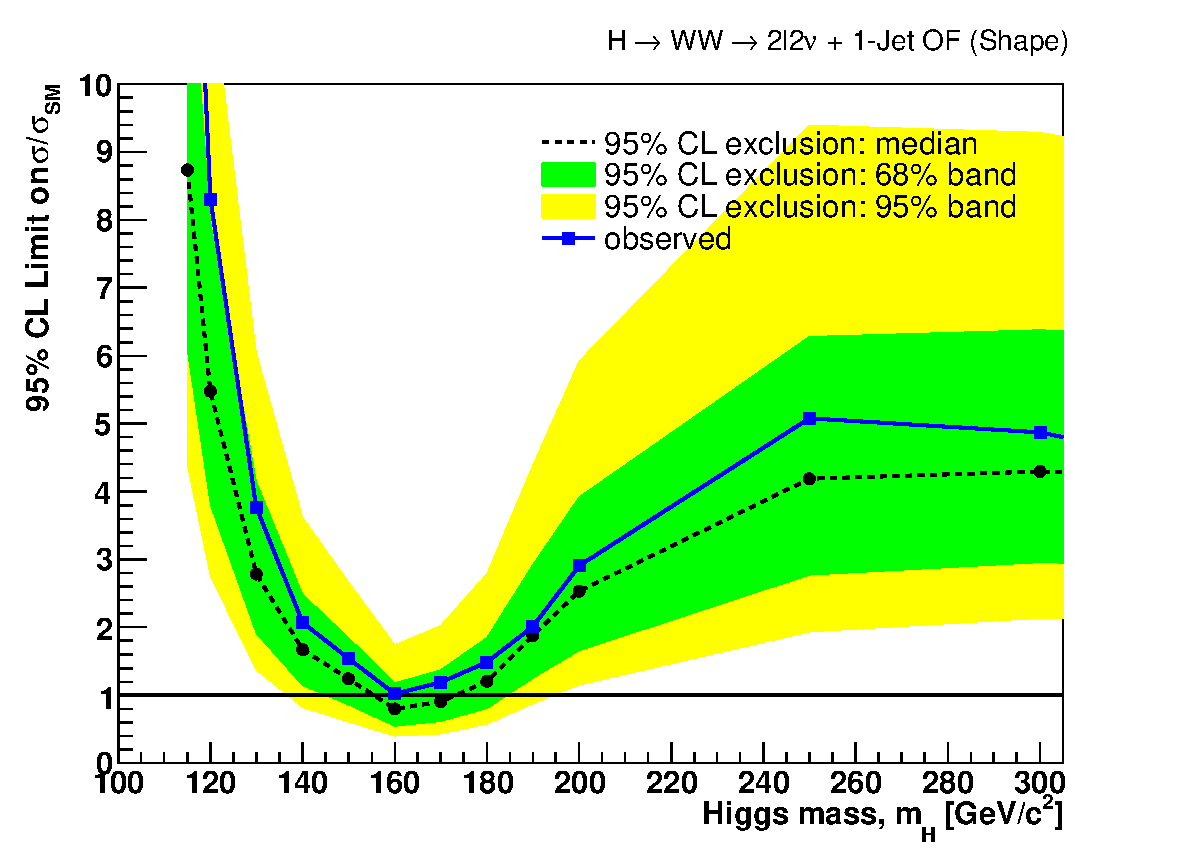
\includegraphics[width=0.48\textwidth]{lp_figures/limits_1j_of_shape_ana_v6_1500pb_LP_EPS.pdf}}
\subfigure[]{
\centering
\label{subfig:post_1j_sf_shape}
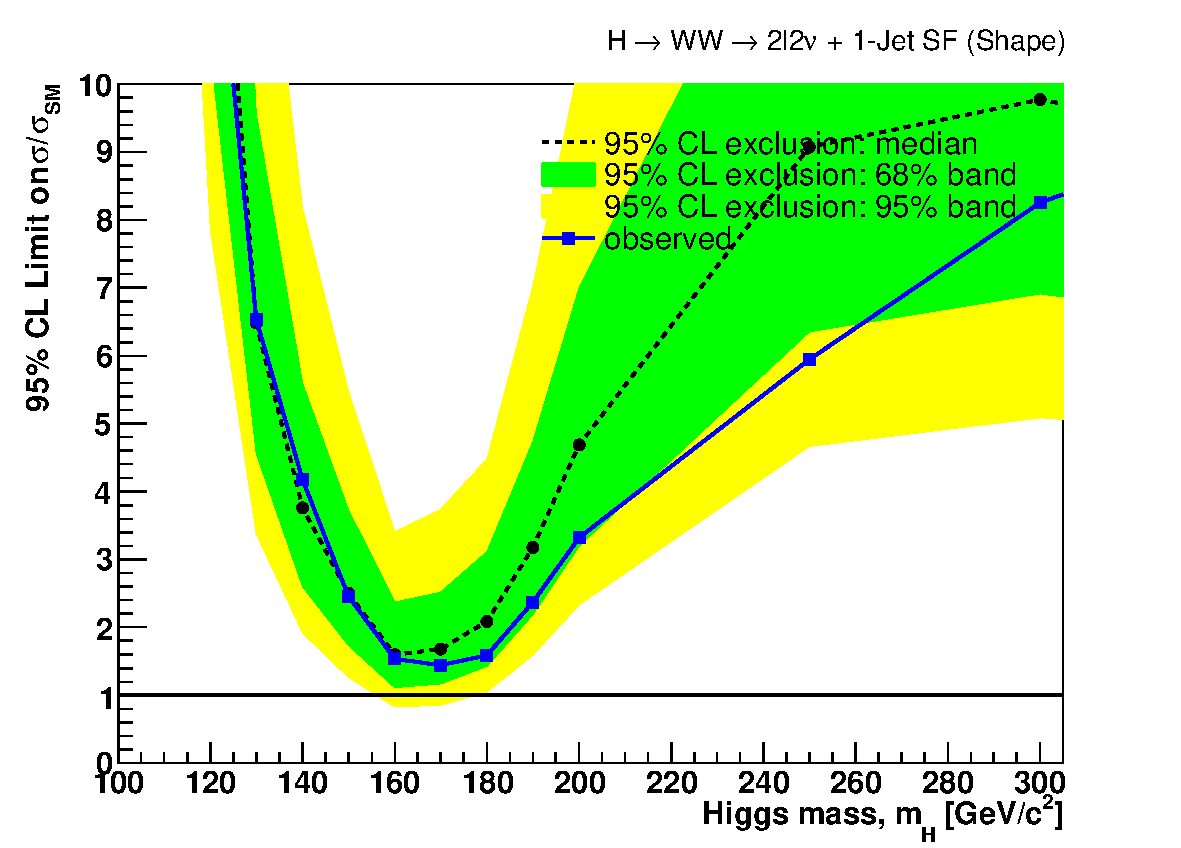
\includegraphics[width=0.48\textwidth]{lp_figures/limits_1j_sf_shape_ana_v6_1500pb_LP_POSTEPS.pdf}}
\subfigure[]{
\centering
\label{subfig:post_1j_of_shape}
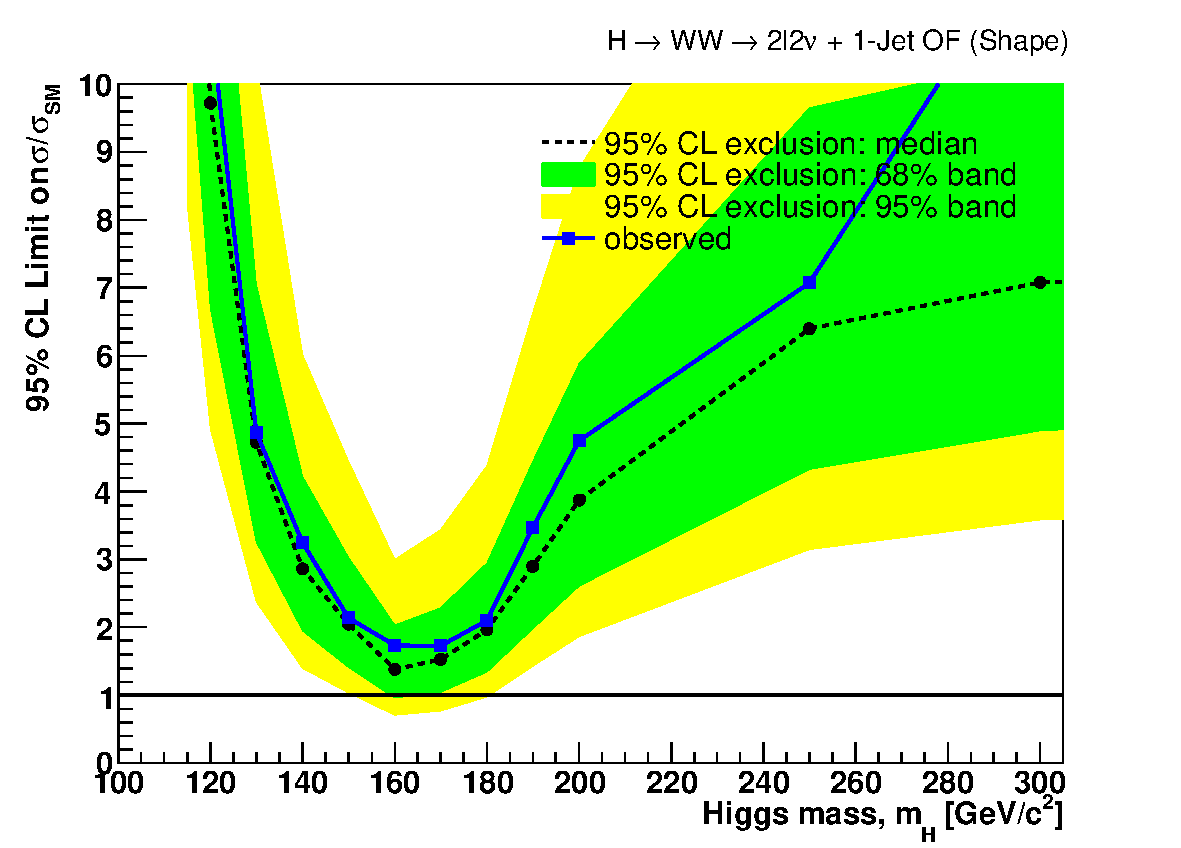
\includegraphics[width=0.48\textwidth]{lp_figures/limits_1j_of_shape_ana_v6_1500pb_LP_POSTEPS.pdf}}
\caption{Multivariate-based analysis upper limits at 95\% C.L. using LP, EPS and post-EPS datasets for 1-jet events.
\subref{subfig:lp_1j_sf_shape}: LP same-flavor; \subref{subfig:lp_1j_of_shape}: LP opposite-flavor;
\subref{subfig:eps_1j_sf_shape}: EPS same-flavor; \subref{subfig:eps_1j_of_shape}: EPS opposite-flavor;
\subref{subfig:post_1j_sf_shape}: post-EPS same-flavor; \subref{subfig:post_1j_of_shape}: post-EPS opposite-flavor;
}
\label{fig:limits_1j_shape}
\end{figure}


%%%%%%%%%%%%%%%%%%%%%%%%%%%%%%
\clearpage
\subsubsection{Cut-Based with Additional Transverse Mass Requirement}
\begin{figure}[!htbp]
\centering
\subfigure[]{
\centering
\label{subfig:0j_sf}
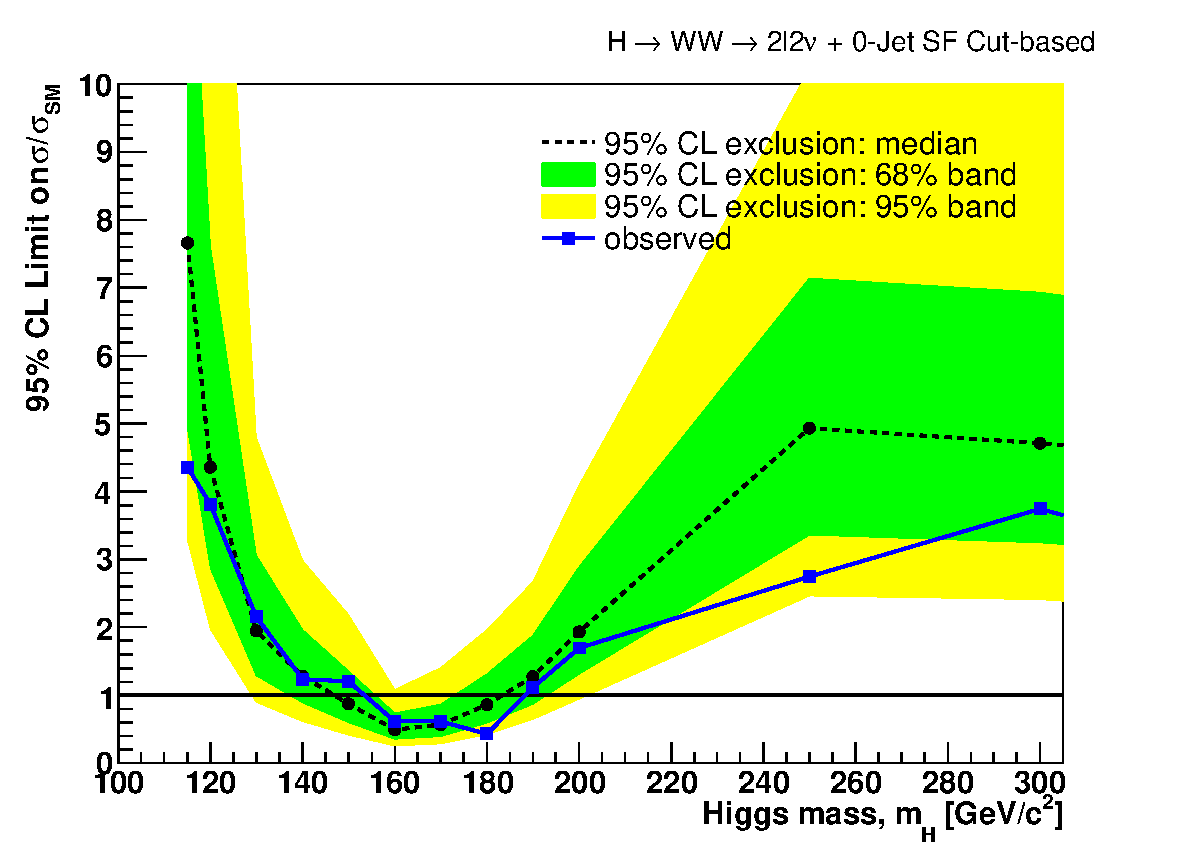
\includegraphics[width=0.48\textwidth]{lp_figures/limits_0j_sf_cut_ana_v6_1500pb_LP_MTCUT80.pdf}}
\subfigure[]{
\centering
\label{subfig:0j_of}
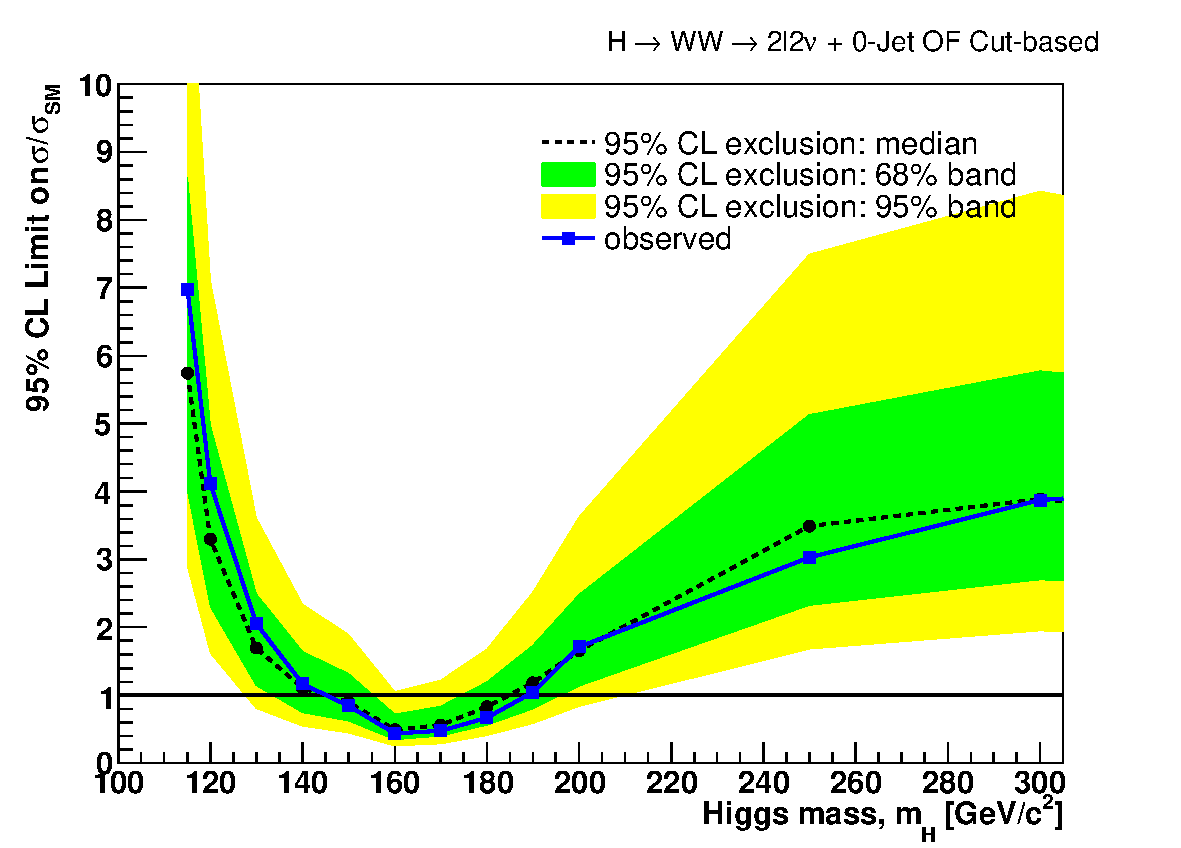
\includegraphics[width=0.48\textwidth]{lp_figures/limits_0j_of_cut_ana_v6_1500pb_LP_MTCUT80.pdf}}
\subfigure[]{
\centering
\label{subfig:1j_sf}
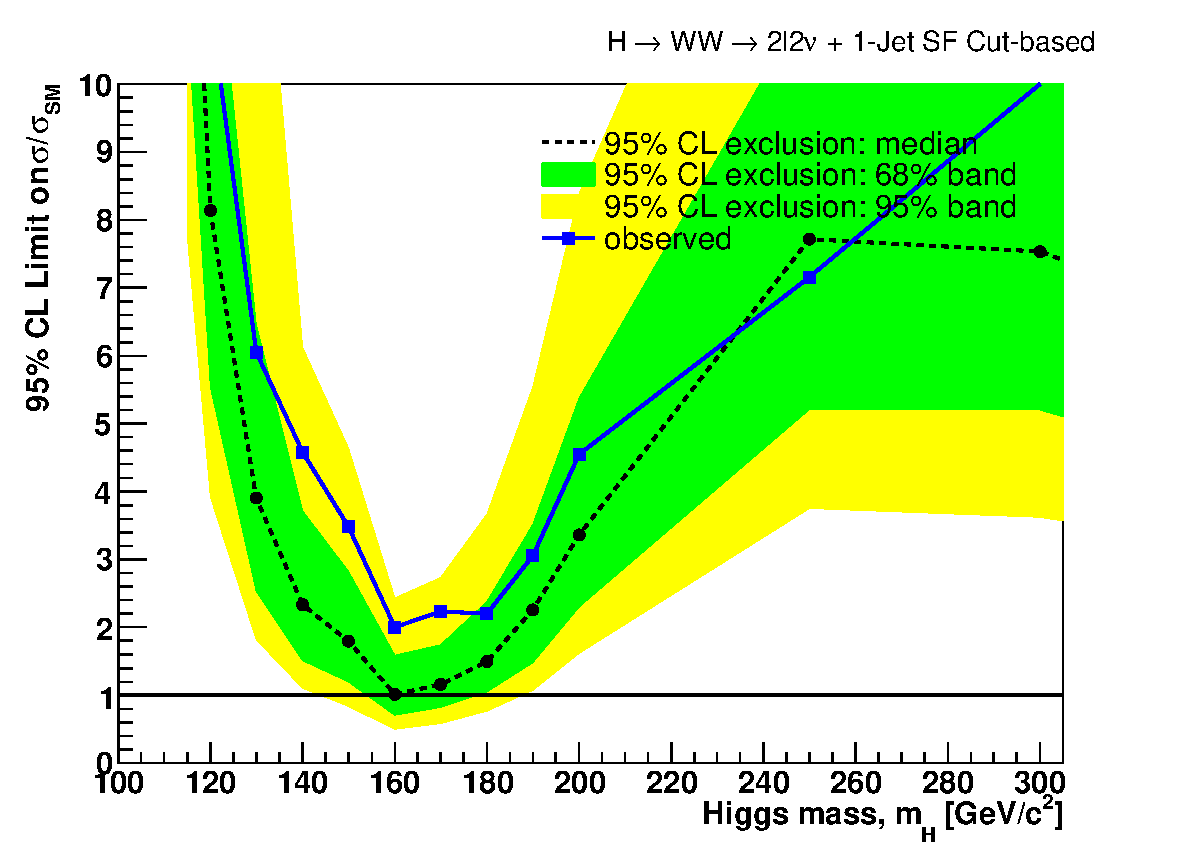
\includegraphics[width=0.48\textwidth]{lp_figures/limits_1j_sf_cut_ana_v6_1500pb_LP_MTCUT80.pdf}}
\subfigure[]{
\centering
\label{subfig:1j_of}
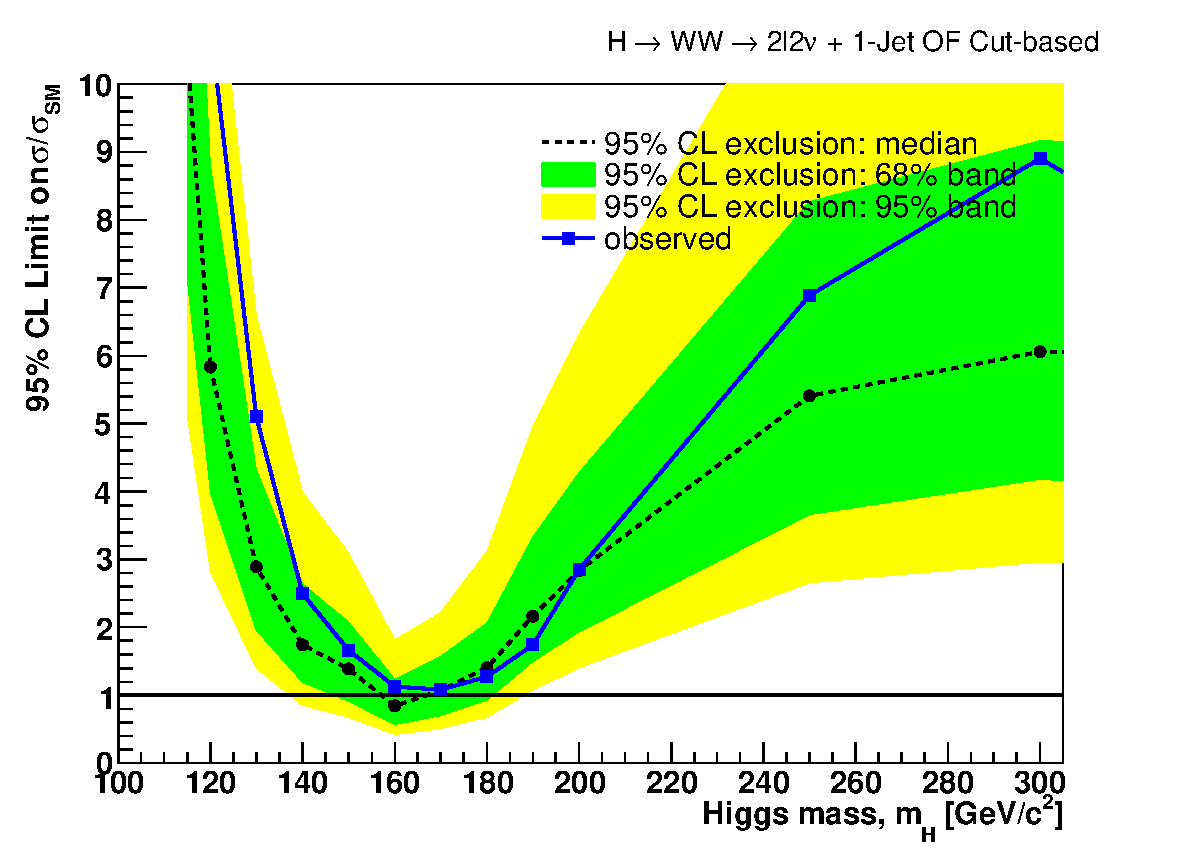
\includegraphics[width=0.48\textwidth]{lp_figures/limits_1j_of_cut_ana_v6_1500pb_LP_MTCUT80.pdf}}
\subfigure[]{
\centering
\label{subfig:2j}
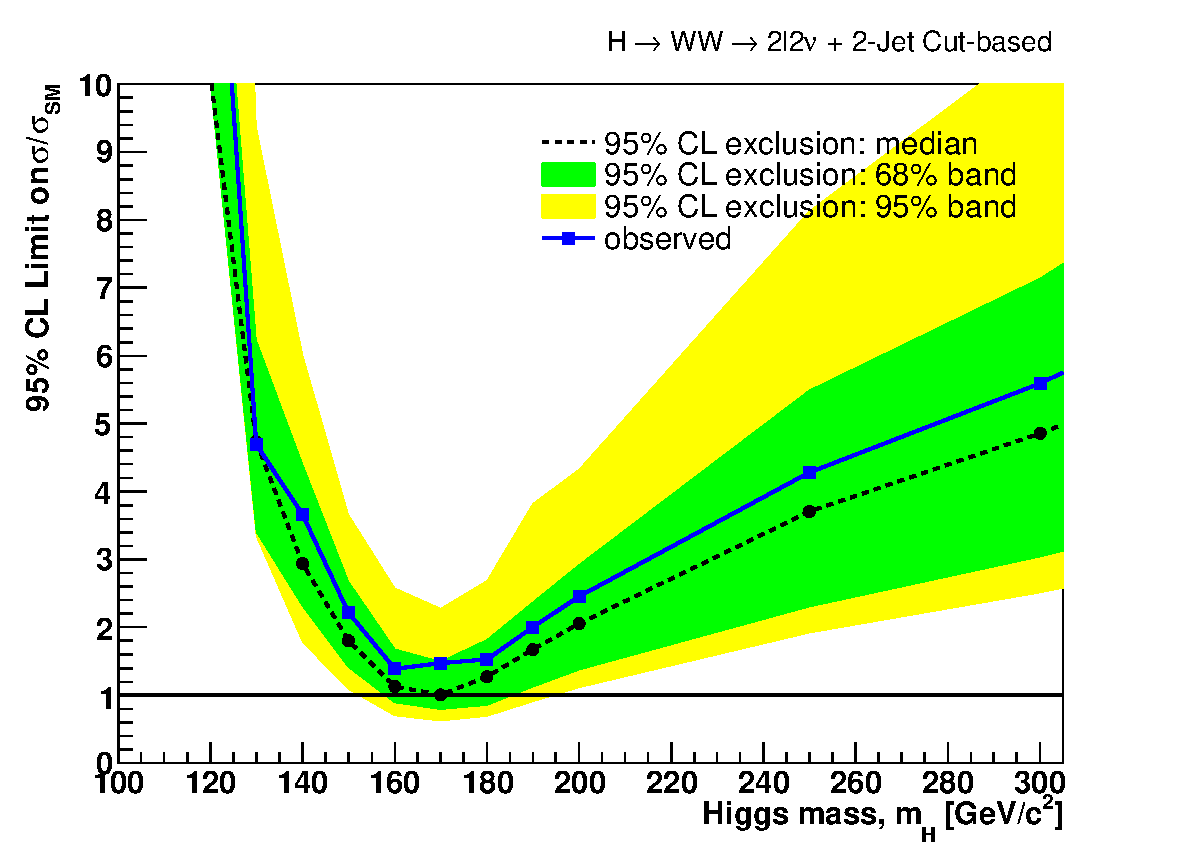
\includegraphics[width=0.48\textwidth]{lp_figures/limits_2j_cut_ana_v6_1500pb_LP_MTCUT80.pdf}}
\subfigure[]{
\centering
\label{subfig:njcomb}
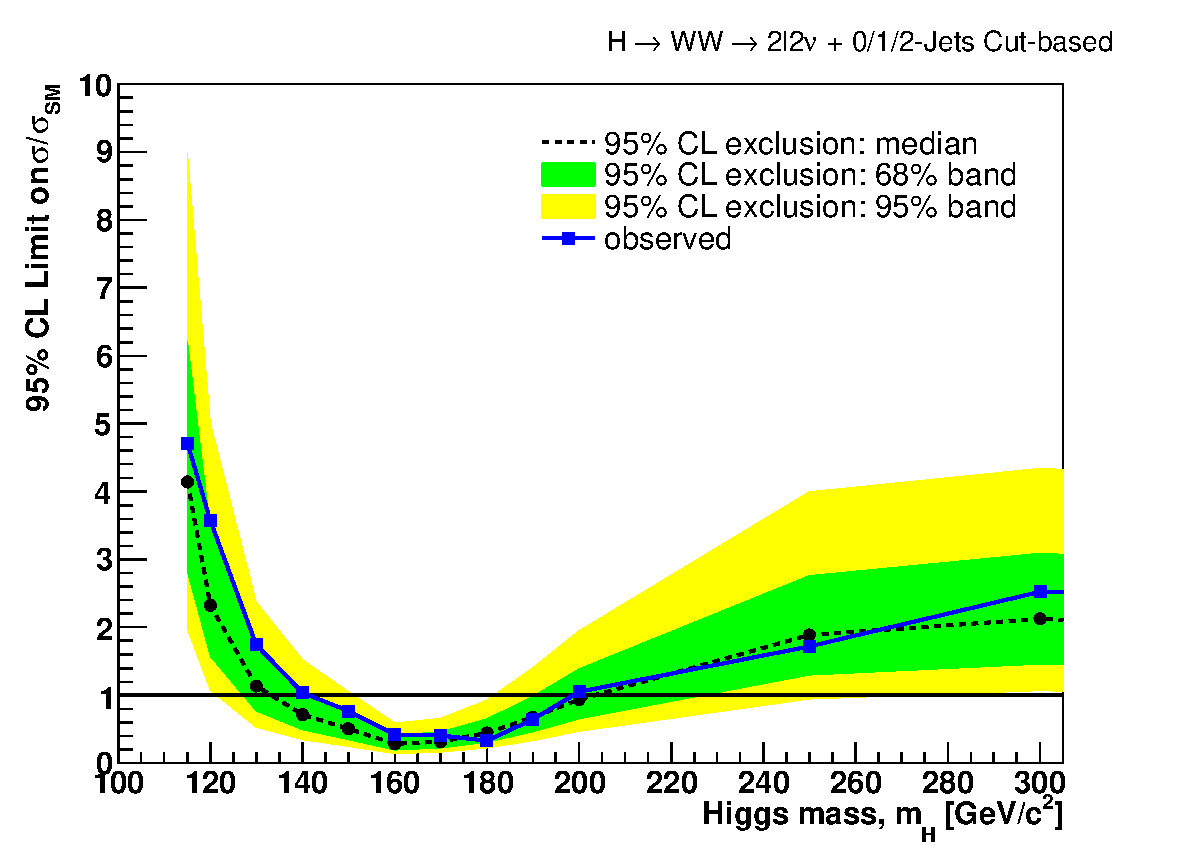
\includegraphics[width=0.48\textwidth]{lp_figures/limits_nj_cut_ana_v6_1500pb_LP_MTCUT80.pdf}}
\caption{Cut-based analysis upper limits at 95\% C.L. using data corresponding to 1.5~$\ifb$ applying the additional $m_T$ cut.
The limits are shown in 4 final states separately. \subref{subfig:0j_sf}: SF in 0 Jet bin;
\subref{subfig:0j_of}: OF in 0 Jet bin; \subref{subfig:1j_sf}: SF in 1 Jet bin;
\subref{subfig:1j_of}: OF in 1 Jet bin; \subref{subfig:2j}: 2 Jet bin; \subref{subfig:njcomb}: 0/1/2 Jets combined; }
\label{fig:limits_lp_mtcut80_cut}
\end{figure}
%%%%%%%%%%%%%%%%%%%%%%%%%%%%%%
\clearpage
\subsubsection{MVA-Based with Additional Transverse Mass Requirement}
\begin{figure}[!htbp]
\centering
\subfigure[]{
\centering
\label{subfig:0j_sf}
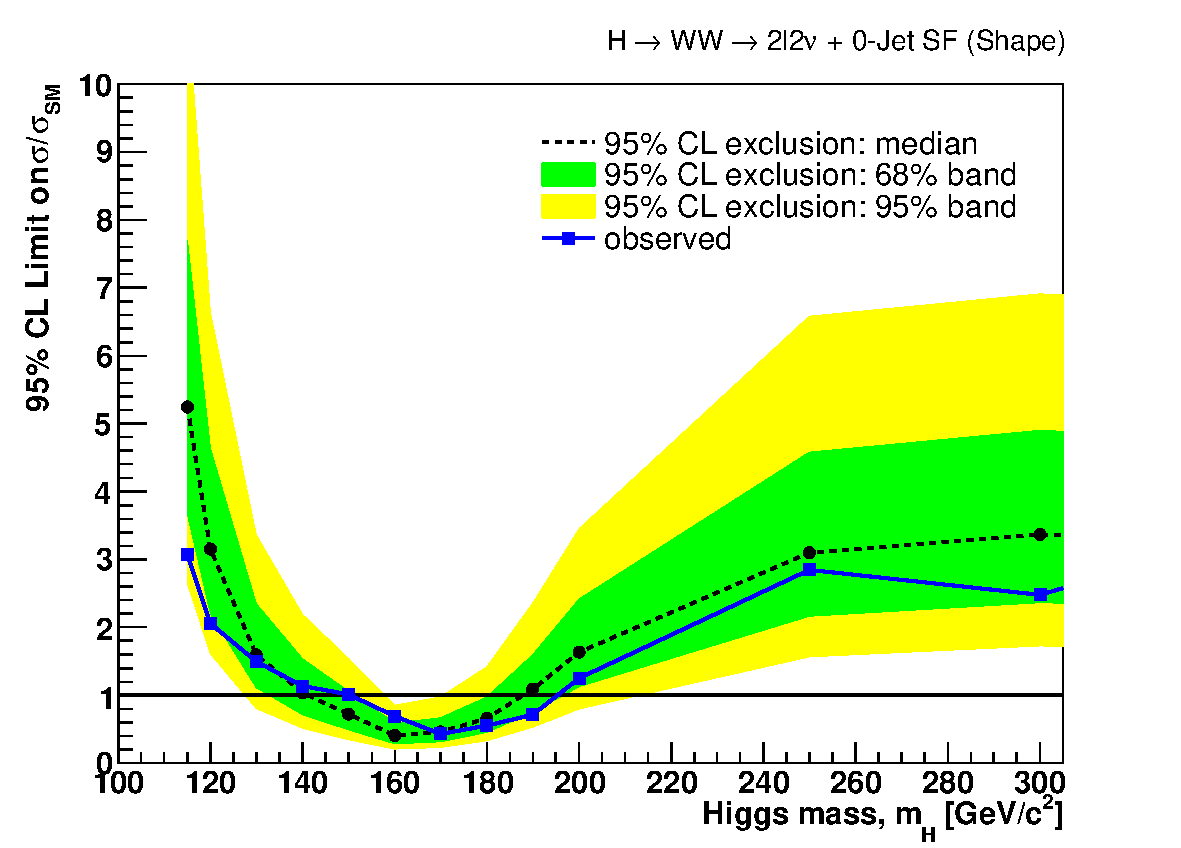
\includegraphics[width=0.48\textwidth]{lp_figures/limits_0j_sf_shape_ana_v6_1500pb_LP_MTCUT80.pdf}
}
\subfigure[]{
\centering
\label{subfig:0j_of}
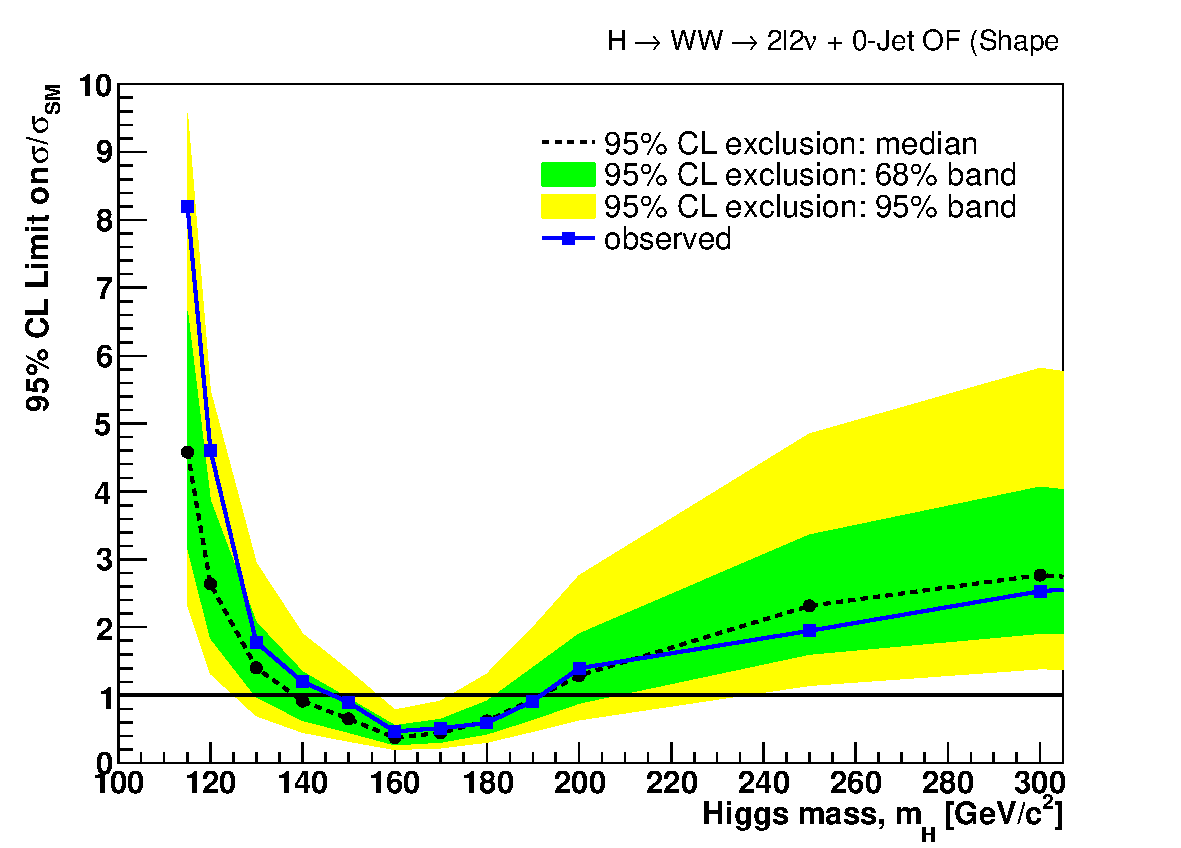
\includegraphics[width=0.48\textwidth]{lp_figures/limits_0j_of_shape_ana_v6_1500pb_LP_MTCUT80.pdf}
}
\subfigure[]{
\centering
\label{subfig:1j_sf}
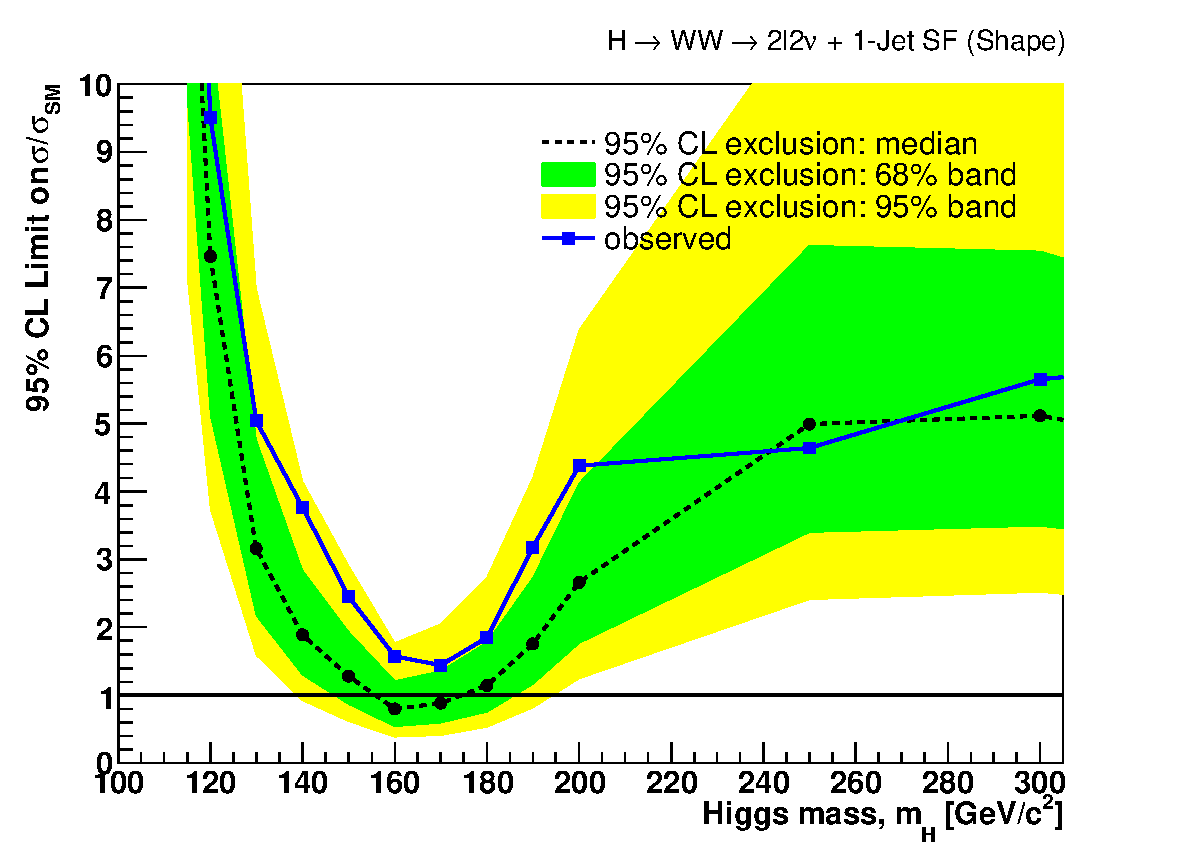
\includegraphics[width=0.48\textwidth]{lp_figures/limits_1j_sf_shape_ana_v6_1500pb_LP_MTCUT80.pdf}
}
\subfigure[]{
\centering
\label{subfig:1j_of}
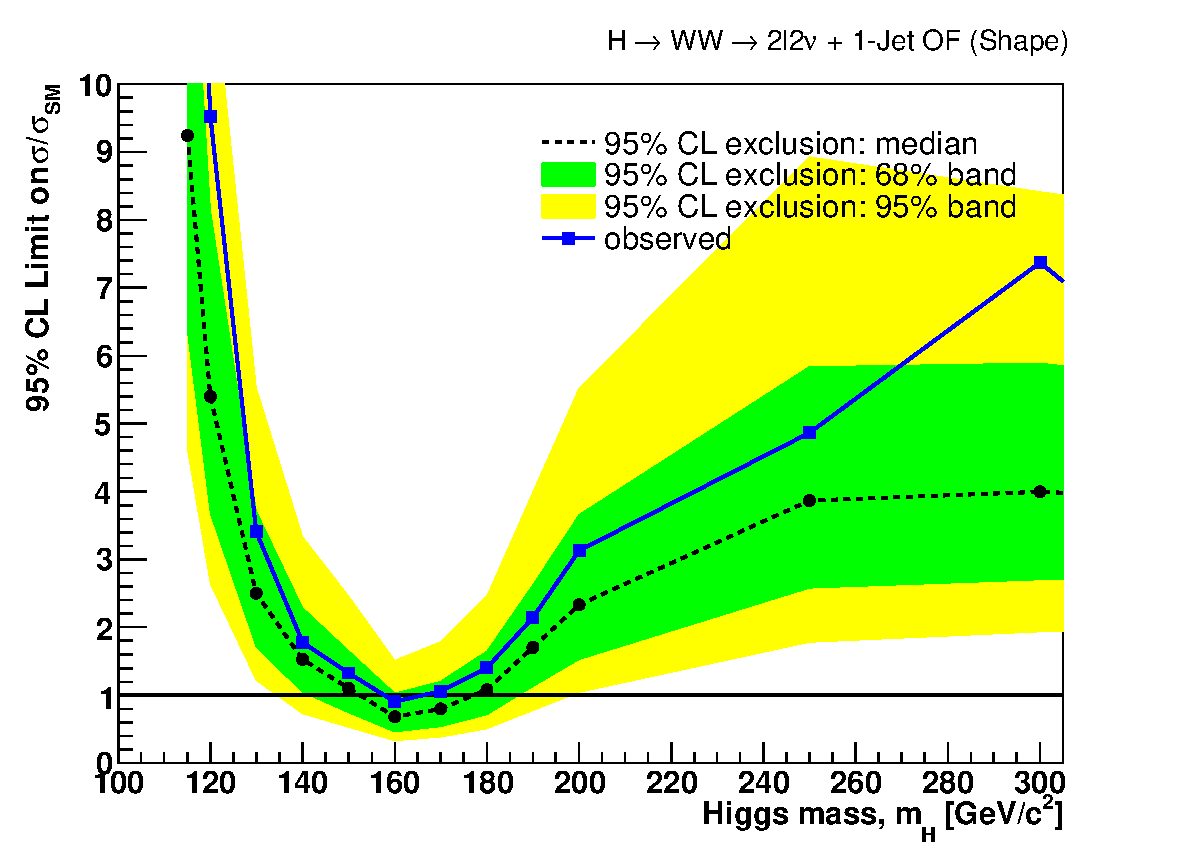
\includegraphics[width=0.48\textwidth]{lp_figures/limits_1j_of_shape_ana_v6_1500pb_LP_MTCUT80.pdf}
}
\subfigure[]{
\centering
\label{subfig:nj}
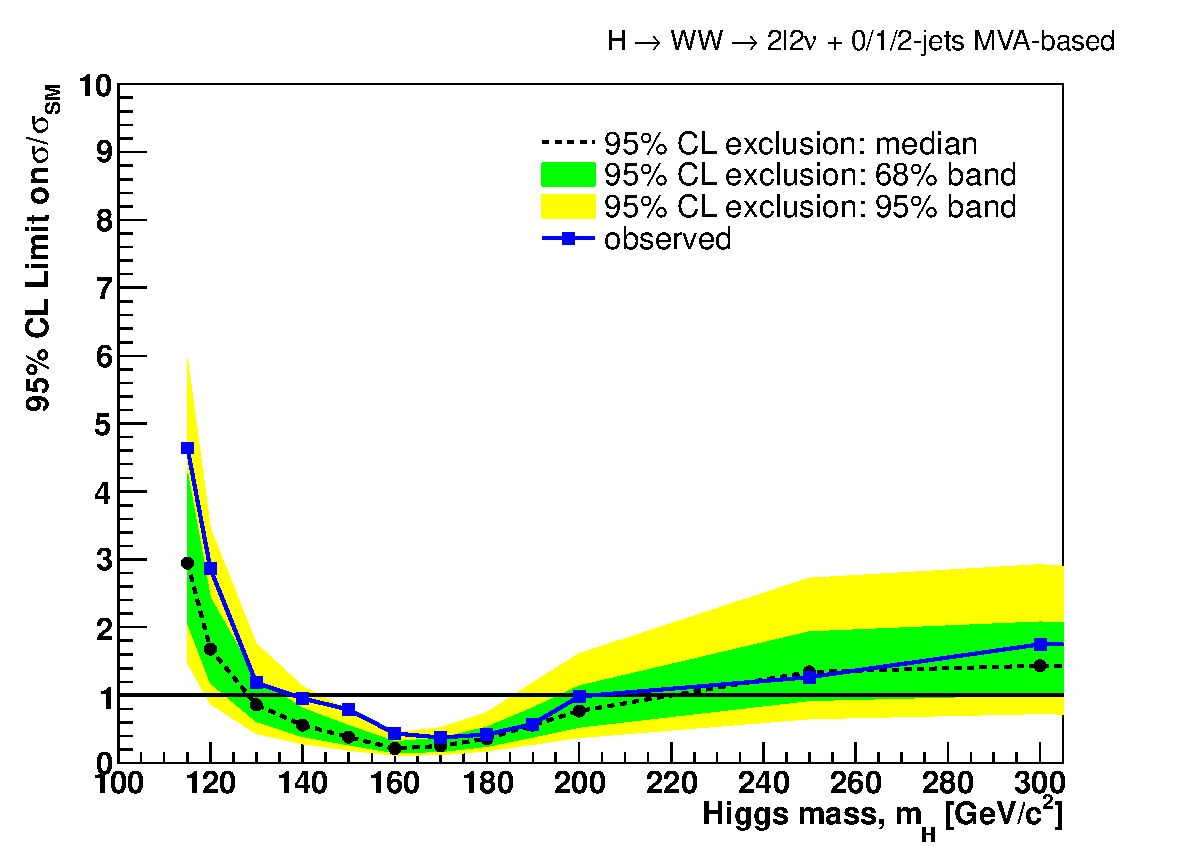
\includegraphics[width=0.48\textwidth]{lp_figures/limits_nj_shape_ana_v6_1500pb_LP_MTCUT80.pdf}
}
\caption{Multivariate based analysis upper limits at 95\% C.L. using data corresponding to 1.5~$\ifb$,
applying the additional $m_T$ cut.
The limits are shown in 4 final states separately. \subref{subfig:0j_sf}: SF in 0 Jet bin;
\subref{subfig:0j_of}: OF in 0 Jet bin; \subref{subfig:1j_sf}: SF in 1 Jet bin;
\subref{subfig:1j_of}: OF in 1 Jet bin; \subref{subfig:nj}: 0/1/2 Jets combined;
}
\label{fig:limits_lp_mtcut80_shape}
\end{figure}

%%%%%%%%%%%%%%%%%%%%%%%%%%%%%%
%
%
%
\pagebreak
\clearpage
\subsection{Tabulated Limits}
\subsubsection{EPS Dataset}
We report the upper limits obtained using the data with the run number
$<170826$ ( referred to as the EPS data) in the 0 and 1 jet bins separating the
same flavor ($ee/\mu\mu$) and opposite flavor ($e\mu$) final states.
The results tabulated in
Table~\ref{tab:limits_eps_cut}-\ref{tab:limits_eps_shape} respectively.

%%%%%%%%%%%%%%%%%%%%%%%%%%%%%%
\begin{table}
\begin{center}
\begin{tabular}{c c c c c}
\hline\hline
 $m_H$ (GeV) & Observed & Median Expected & 68\% C.L. Band & 95\% C.L. Band \\ \hline
\hline
\multicolumn{5}{c} {0-Jet Bin Same Flavor} \\
\hline
115 & 4.1 & 8.8 & [5.7, 15.4] & [4.0, 36.0] \\
120 & 4.1 & 5.0 & [3.2, 8.4] & [2.3, 17.6] \\
130 & 2.5 & 2.3 & [1.5, 3.4] & [1.0, 5.4] \\
140 & 1.6 & 1.5 & [1.0, 2.2] & [0.7, 3.3] \\
150 & 1.8 & 1.0 & [0.7, 1.5] & [0.5, 2.4] \\
160 & 1.0 & 0.6 & [0.4, 0.9] & [0.3, 1.6] \\
170 & 1.0 & 0.7 & [0.5, 1.0] & [0.3, 1.6] \\
180 & 0.6 & 1.0 & [0.7, 1.5] & [0.5, 2.2] \\
190 & 1.6 & 1.5 & [1.0, 2.1] & [0.7, 3.1] \\
200 & 2.1 & 2.2 & [1.6, 3.3] & [1.1, 4.6] \\
250 & 3.3 & 5.8 & [4.0, 8.5] & [3.0, 12.2] \\
300 & 4.3 & 5.5 & [3.9, 8.3] & [2.8, 11.9] \\
\hline
\multicolumn{5}{c} {0-Jet Bin Opposite Flavor} \\
\hline
115 & 7.6 & 6.6 & [4.5, 9.8] & [3.2, 14.4] \\
120 & 4.9 & 3.8 & [2.6, 5.7] & [1.9, 8.2] \\
130 & 2.8 & 1.9 & [1.3, 2.9] & [1.0, 4.2] \\
140 & 1.5 & 1.3 & [0.9, 1.8] & [0.6, 2.6] \\
150 & 0.9 & 1.0 & [0.7, 1.5] & [0.5, 2.2] \\
160 & 0.5 & 0.5 & [0.4, 0.8] & [0.3, 1.2] \\
170 & 0.7 & 0.7 & [0.5, 1.0] & [0.3, 1.4] \\
180 & 0.9 & 0.9 & [0.7, 1.4] & [0.5, 2.0] \\
190 & 1.4 & 1.3 & [0.9, 2.0] & [0.7, 2.8] \\
200 & 2.3 & 1.9 & [1.3, 2.8] & [1.0, 4.2] \\
250 & 3.1 & 3.9 & [2.8, 5.8] & [2.0, 8.2] \\
300 & 3.8 & 4.5 & [3.1, 6.6] & [2.3, 9.5] \\
\hline
\multicolumn{5}{c} {1-Jet Bin Same Flavor} \\
\hline
115 & 19.7 & 17.7 & [11.4, 26.5] & [8.6, 43.9] \\
120 & 12.4 & 9.4 & [6.4, 15.3] & [4.7, 27.8] \\
130 & 8.3 & 4.6 & [3.1, 7.2] & [2.1, 14.5] \\
140 & 5.7 & 2.7 & [1.7, 4.1] & [1.2, 7.0] \\
150 & 4.2 & 2.1 & [1.3, 3.2] & [1.0, 5.2] \\
160 & 2.3 & 1.1 & [0.8, 1.8] & [0.6, 2.7] \\
170 & 2.7 & 1.4 & [1.0, 2.1] & [0.7, 3.2] \\
180 & 2.9 & 1.8 & [1.3, 2.6] & [0.9, 3.8] \\
190 & 4.3 & 2.6 & [1.7, 4.0] & [1.3, 6.1] \\
200 & 6.5 & 4.0 & [2.7, 6.0] & [2.0, 9.4] \\
250 & 11.2 & 8.6 & [6.0, 13.2] & [4.4, 19.7] \\
300 & 12.1 & 8.7 & [6.0, 13.1] & [4.3, 19.5] \\
\hline
\multicolumn{5}{c} {1-Jet Bin Opposite Flavor} \\
\hline
115 & 19.4 & 10.2 & [6.9, 15.4] & [5.1, 22.9] \\
120 & 10.4 & 6.0 & [4.0, 8.9] & [3.0, 13.0] \\
130 & 4.1 & 3.2 & [2.1, 4.7] & [1.5, 7.2] \\
140 & 2.2 & 2.0 & [1.4, 3.0] & [1.0, 4.6] \\
150 & 1.6 & 1.6 & [1.1, 2.3] & [0.8, 3.5] \\
160 & 1.1 & 1.0 & [0.6, 1.4] & [0.5, 2.1] \\
170 & 1.2 & 1.2 & [0.8, 1.7] & [0.6, 2.7] \\
180 & 1.6 & 1.6 & [1.1, 2.5] & [0.9, 3.6] \\
190 & 2.1 & 2.6 & [1.8, 3.8] & [1.3, 5.6] \\
200 & 3.1 & 3.2 & [2.2, 4.8] & [1.6, 7.1] \\
250 & 6.2 & 6.1 & [4.2, 9.1] & [3.1, 13.6] \\
300 & 7.8 & 6.9 & [4.8, 10.4] & [3.5, 15.2] \\
\hline\hline
\end{tabular}
\end{center}
\caption{Cut based upper limits at 95\% C.L. in 0 and 1 Jet final state,
using the EPS data (run $<$ 170826) corresponding to  1.1~$\ifb$.}
\label{tab:limits_eps_cut}
\end{table}
%%%%%%%%%%%%%%%%%%%%%%%%%%%%%%
%%%%%%%%%%%%%%%%%%%%%%%%%%%%%%
\begin{table}
\begin{center}
\begin{tabular}{c c c c c}
\hline\hline
 $m_H$ (GeV) & Observed & Median Expected & 68\% C.L. Band & 95\% C.L. Band \\ \hline
\hline
\multicolumn{5}{c} {0-Jet Bin Same Flavor} \\
\hline
115 & 3.7 & 6.0 & [4.2, 8.7] & [3.1, 12.6] \\
120 & 2.6 & 3.6 & [2.5, 5.2] & [1.8, 7.5] \\
130 & 2.1 & 1.8 & [1.2, 2.6] & [0.9, 3.7] \\
140 & 1.9 & 1.2 & [0.8, 1.7] & [0.6, 2.4] \\
150 & 1.5 & 0.8 & [0.6, 1.2] & [0.4, 1.7] \\
160 & 1.0 & 0.5 & [0.3, 0.7] & [0.2, 1.0] \\
170 & 0.7 & 0.5 & [0.4, 0.8] & [0.3, 1.1] \\
180 & 0.8 & 0.7 & [0.5, 1.1] & [0.4, 1.6] \\
190 & 1.0 & 1.2 & [0.8, 1.8] & [0.6, 2.6] \\
200 & 1.5 & 1.8 & [1.3, 2.7] & [0.9, 3.9] \\
250 & 3.0 & 3.5 & [2.5, 5.2] & [1.8, 7.5] \\
300 & 3.5 & 3.9 & [2.8, 5.8] & [2.0, 8.2] \\
\hline
\multicolumn{5}{c} {0-Jet Bin Opposite Flavor} \\
\hline
115 & 10.9 & 5.0 & [3.4, 7.3] & [2.5, 10.5] \\
120 & 5.9 & 2.9 & [2.0, 4.3] & [1.4, 5.9] \\
130 & 2.4 & 1.5 & [1.1, 2.2] & [0.8, 3.2] \\
140 & 1.3 & 1.0 & [0.7, 1.4] & [0.5, 2.1] \\
150 & 1.1 & 0.7 & [0.5, 1.0] & [0.4, 1.5] \\
160 & 0.7 & 0.4 & [0.3, 0.6] & [0.2, 0.9] \\
170 & 0.7 & 0.5 & [0.3, 0.7] & [0.3, 1.1] \\
180 & 0.8 & 0.7 & [0.5, 1.0] & [0.4, 1.5] \\
190 & 1.3 & 1.1 & [0.7, 1.6] & [0.5, 2.2] \\
200 & 1.8 & 1.4 & [1.0, 2.1] & [0.7, 3.0] \\
250 & 2.2 & 2.6 & [1.8, 3.7] & [1.3, 5.3] \\
300 & 2.7 & 3.2 & [2.2, 4.7] & [1.6, 6.6] \\
\hline
\multicolumn{5}{c} {1-Jet Bin Same Flavor} \\
\hline
115 & 24.4 & 14.8 & [10.3, 21.7] & [7.5, 30.8] \\
120 & 11.5 & 8.3 & [5.7, 12.2] & [4.2, 17.9] \\
130 & 6.5 & 3.7 & [2.5, 5.5] & [1.8, 7.8] \\
140 & 4.1 & 2.1 & [1.5, 3.1] & [1.1, 4.6] \\
150 & 2.6 & 1.4 & [1.0, 2.2] & [0.7, 3.2] \\
160 & 1.6 & 0.9 & [0.6, 1.3] & [0.4, 2.0] \\
170 & 1.8 & 1.0 & [0.7, 1.5] & [0.5, 2.3] \\
180 & 2.5 & 1.3 & [0.8, 1.9] & [0.6, 2.9] \\
190 & 4.0 & 2.0 & [1.3, 3.0] & [0.9, 4.6] \\
200 & 5.8 & 3.0 & [2.0, 4.6] & [1.4, 6.9] \\
250 & 6.7 & 5.6 & [3.8, 8.4] & [2.7, 12.5] \\
300 & 7.2 & 5.8 & [4.0, 8.5] & [2.9, 12.2] \\
\hline
\multicolumn{5}{c} {1-Jet Bin Opposite Flavor} \\
\hline
115 & 15.8 & 8.7 & [6.1, 12.8] & [4.4, 18.3] \\
120 & 8.3 & 5.5 & [3.8, 8.0] & [2.8, 11.6] \\
130 & 3.8 & 2.8 & [1.9, 4.2] & [1.4, 6.0] \\
140 & 2.1 & 1.7 & [1.1, 2.5] & [0.8, 3.6] \\
150 & 1.5 & 1.2 & [0.9, 1.9] & [0.6, 2.7] \\
160 & 1.0 & 0.8 & [0.5, 1.2] & [0.4, 1.7] \\
170 & 1.2 & 0.9 & [0.6, 1.4] & [0.4, 2.0] \\
180 & 1.5 & 1.2 & [0.8, 1.8] & [0.6, 2.8] \\
190 & 2.0 & 1.9 & [1.2, 2.9] & [0.9, 4.4] \\
200 & 2.9 & 2.5 & [1.7, 3.9] & [1.2, 5.9] \\
250 & 5.1 & 4.2 & [2.8, 6.3] & [1.9, 9.4] \\
300 & 4.9 & 4.3 & [3.0, 6.4] & [2.1, 9.3] \\
\hline\hline
\end{tabular}
\end{center}
\caption{Multivariate based upper limits at 95\% C.L. in 0 and 1 Jet final state,
using the EPS data (run $<$ 170826) corresponding to  1.1~$\ifb$.}
\label{tab:limits_eps_shape}
\end{table}
%%%%%%%%%%%%%%%%%%%%%%%%%%%%%%

%
%
%
\pagebreak
\clearpage
\subsubsection{post-EPS Dataset}
We report the upper limits obtained using the data with the run number $>=170826$ ( referred to
as the post-EPS data) in the 0 and 1 jet bins separating the
same flavor ($ee/\mu\mu$) and opposite flavor ($e\mu$) final states.
The results are tabulated in
Table~\ref{tab:limits_posteps_cut}-\ref{tab:limits_posteps_shape} respectively.

%%%%%%%%%%%%%%%%%%%%%%%%%%%%%%
\begin{table}
\begin{center}
\begin{tabular}{c c c c c}
\hline\hline
 $m_H$ (GeV) & Observed & Median Expected & 68\% C.L. Band & 95\% C.L. Band \\ \hline
\hline
\multicolumn{5}{c} {0-Jet Bin Same Flavor} \\
\hline
115 & 14.3 & 12.9 & [8.8, 21.4] & [6.8, 43.3] \\
120 & 6.9 & 7.6 & [5.0, 11.9] & [3.6, 21.3] \\
130 & 3.1 & 3.4 & [2.3, 5.2] & [1.7, 7.5] \\
140 & 1.8 & 2.3 & [1.6, 3.4] & [1.2, 5.0] \\
150 & 1.1 & 1.7 & [1.1, 2.5] & [1.0, 3.8] \\
160 & 0.6 & 1.0 & [0.7, 1.5] & [0.6, 2.2] \\
170 & 0.6 & 1.2 & [0.9, 1.7] & [0.6, 2.5] \\
180 & 1.0 & 1.9 & [1.4, 2.5] & [1.0, 3.7] \\
190 & 1.6 & 2.6 & [1.8, 3.9] & [1.4, 5.3] \\
200 & 3.2 & 3.8 & [2.8, 5.4] & [2.1, 7.9] \\
250 & 8.1 & 9.5 & [6.9, 14.4] & [5.2, 20.2] \\
300 & 9.5 & 9.5 & [7.0, 14.4] & [5.1, 20.2] \\
\hline
\multicolumn{5}{c} {0-Jet Bin Opposite Flavor} \\
\hline
115 & 9.6 & 10.4 & [7.2, 15.1] & [5.2, 22.3] \\
120 & 4.9 & 5.8 & [4.1, 8.6] & [3.0, 12.8] \\
130 & 2.6 & 3.0 & [2.1, 4.5] & [1.5, 6.3] \\
140 & 1.6 & 2.0 & [1.4, 2.9] & [1.1, 4.1] \\
150 & 1.9 & 1.7 & [1.3, 2.5] & [0.9, 3.7] \\
160 & 0.9 & 1.0 & [0.7, 1.5] & [0.6, 2.2] \\
170 & 0.7 & 1.3 & [0.9, 1.7] & [0.6, 2.6] \\
180 & 1.2 & 1.6 & [1.2, 2.5] & [1.0, 3.3] \\
190 & 1.6 & 2.4 & [1.6, 3.4] & [1.2, 4.7] \\
200 & 2.4 & 3.4 & [2.4, 4.8] & [1.7, 6.6] \\
250 & 7.7 & 6.8 & [4.8, 9.6] & [3.5, 13.7] \\
300 & 10.4 & 8.1 & [5.4, 11.7] & [4.2, 16.0] \\
\hline
\multicolumn{5}{c} {1-Jet Bin Same Flavor} \\
\hline
115 & 37.5 & 31.2 & [21.4, 50.3] & [17.2, 74.9] \\
120 & 19.1 & 16.3 & [11.7, 25.6] & [9.4, 42.9] \\
130 & 7.5 & 8.7 & [6.3, 13.2] & [4.5, 21.9] \\
140 & 5.2 & 5.1 & [3.5, 7.2] & [2.5, 11.4] \\
150 & 4.5 & 3.7 & [2.6, 5.4] & [2.1, 9.0] \\
160 & 2.9 & 2.4 & [1.6, 3.4] & [1.3, 5.1] \\
170 & 3.1 & 2.5 & [2.0, 3.8] & [1.6, 5.3] \\
180 & 3.0 & 3.1 & [2.4, 4.5] & [1.9, 7.0] \\
190 & 3.3 & 4.7 & [3.3, 6.6] & [2.4, 9.9] \\
200 & 4.9 & 7.0 & [4.9, 10.8] & [4.0, 15.4] \\
250 & 9.2 & 15.3 & [11.0, 23.8] & [9.1, 34.2] \\
300 & 16.0 & 15.9 & [11.5, 21.6] & [8.5, 30.9] \\
\hline
\multicolumn{5}{c} {1-Jet Bin Opposite Flavor} \\
\hline
115 & 41.3 & 19.6 & [14.2, 29.5] & [10.4, 41.5] \\
120 & 24.8 & 11.2 & [7.4, 16.5] & [5.6, 24.4] \\
130 & 11.4 & 5.6 & [3.7, 8.2] & [3.1, 11.5] \\
140 & 6.4 & 3.7 & [2.7, 5.6] & [2.0, 8.0] \\
150 & 4.2 & 3.0 & [2.1, 4.2] & [1.5, 6.1] \\
160 & 2.6 & 1.8 & [1.2, 2.6] & [1.0, 3.9] \\
170 & 2.6 & 2.2 & [1.7, 3.2] & [1.4, 5.0] \\
180 & 2.6 & 3.2 & [2.2, 4.6] & [1.7, 6.2] \\
190 & 3.7 & 4.4 & [3.2, 6.6] & [2.4, 9.3] \\
200 & 6.3 & 5.5 & [4.1, 8.1] & [3.1, 12.2] \\
250 & 17.0 & 9.9 & [7.0, 15.2] & [5.4, 21.8] \\
300 & 21.4 & 11.2 & [8.4, 17.3] & [6.0, 24.9] \\
\hline\hline
\end{tabular}
\end{center}
\caption{Cut-based upper limits at 95\% C.L. in 0 and 1 Jet final state,
using the post-EPS data (run $>=$ 170826) corresponding to  0.4~$\ifb$.}
\label{tab:limits_posteps_cut}
\end{table}
%%%%%%%%%%%%%%%%%%%%%%%%%%%%%%
%%%%%%%%%%%%%%%%%%%%%%%%%%%%%%
\begin{table}
\begin{center}
\begin{tabular}{c c c c c}
\hline\hline
 $m_H$ (GeV) & Observed & Median Expected & 68\% C.L. Band & 95\% C.L. Band \\ \hline
\hline
\multicolumn{5}{c} {0-Jet Bin Same Flavor} \\
\hline
115 & 10.2 & 10.2 & [7.3, 14.7] & [5.4, 20.9] \\
120 & 4.8 & 5.9 & [4.2, 8.5] & [3.1, 12.4] \\
130 & 2.7 & 2.8 & [2.0, 4.1] & [1.5, 5.9] \\
140 & 1.2 & 1.8 & [1.2, 2.6] & [0.9, 3.7] \\
150 & 0.8 & 1.2 & [0.9, 1.8] & [0.6, 2.6] \\
160 & 0.5 & 0.8 & [0.6, 1.1] & [0.4, 1.6] \\
170 & 0.5 & 0.9 & [0.6, 1.2] & [0.4, 1.8] \\
180 & 0.8 & 1.2 & [0.8, 1.8] & [0.6, 2.5] \\
190 & 1.5 & 1.9 & [1.3, 2.8] & [1.0, 4.1] \\
200 & 2.6 & 2.9 & [2.0, 4.2] & [1.5, 6.1] \\
250 & 6.9 & 5.9 & [4.1, 8.6] & [3.0, 12.3] \\
300 & 5.2 & 6.7 & [4.7, 9.8] & [3.6, 14.0] \\
\hline
\multicolumn{5}{c} {0-Jet Bin Opposite Flavor} \\
\hline
115 & 9.8 & 7.9 & [5.5, 11.5] & [4.1, 16.5] \\
120 & 4.8 & 4.7 & [3.3, 6.9] & [2.4, 9.8] \\
130 & 3.3 & 2.4 & [1.7, 3.6] & [1.2, 5.2] \\
140 & 2.0 & 1.6 & [1.1, 2.4] & [0.8, 3.4] \\
150 & 1.8 & 1.2 & [0.8, 1.7] & [0.6, 2.4] \\
160 & 0.9 & 0.8 & [0.5, 1.1] & [0.4, 1.6] \\
170 & 0.9 & 0.9 & [0.6, 1.2] & [0.4, 1.8] \\
180 & 1.0 & 1.2 & [0.8, 1.7] & [0.6, 2.4] \\
190 & 1.5 & 1.7 & [1.2, 2.5] & [0.8, 3.5] \\
200 & 1.9 & 2.3 & [1.6, 3.4] & [1.2, 4.9] \\
250 & 4.9 & 4.3 & [3.0, 6.2] & [2.2, 8.9] \\
300 & 6.4 & 5.2 & [3.7, 7.7] & [2.7, 10.9] \\
\hline
\multicolumn{5}{c} {1-Jet Bin Same Flavor} \\
\hline
115 & 26.5 & 26.2 & [18.5, 38.7] & [14.1, 55.0] \\
120 & 13.4 & 15.0 & [10.5, 22.0] & [7.9, 32.3] \\
130 & 6.5 & 6.5 & [4.6, 9.6] & [3.4, 13.9] \\
140 & 4.2 & 3.8 & [2.6, 5.6] & [1.9, 8.2] \\
150 & 2.5 & 2.5 & [1.7, 3.7] & [1.3, 5.5] \\
160 & 1.5 & 1.6 & [1.1, 2.4] & [0.8, 3.4] \\
170 & 1.4 & 1.7 & [1.2, 2.5] & [0.9, 3.7] \\
180 & 1.6 & 2.1 & [1.4, 3.1] & [1.0, 4.5] \\
190 & 2.4 & 3.2 & [2.2, 4.7] & [1.6, 7.0] \\
200 & 3.3 & 4.7 & [3.2, 7.0] & [2.3, 10.3] \\
250 & 5.9 & 9.1 & [6.3, 13.6] & [4.7, 19.9] \\
300 & 8.3 & 9.8 & [6.9, 14.4] & [5.1, 20.9] \\
\hline
\multicolumn{5}{c} {1-Jet Bin Opposite Flavor} \\
\hline
115 & 20.2 & 15.9 & [11.1, 23.5] & [8.2, 33.6] \\
120 & 11.0 & 9.7 & [6.7, 14.3] & [4.9, 20.9] \\
130 & 4.9 & 4.7 & [3.3, 7.1] & [2.4, 10.3] \\
140 & 3.2 & 2.9 & [2.0, 4.2] & [1.4, 6.0] \\
150 & 2.1 & 2.0 & [1.4, 3.0] & [1.0, 4.4] \\
160 & 1.7 & 1.4 & [1.0, 2.0] & [0.7, 3.0] \\
170 & 1.7 & 1.5 & [1.0, 2.3] & [0.8, 3.4] \\
180 & 2.1 & 2.0 & [1.3, 2.9] & [1.0, 4.4] \\
190 & 3.5 & 2.9 & [2.0, 4.4] & [1.4, 6.6] \\
200 & 4.7 & 3.9 & [2.6, 5.9] & [1.9, 8.8] \\
250 & 7.1 & 6.4 & [4.3, 9.6] & [3.1, 14.1] \\
300 & 12.3 & 7.1 & [4.9, 10.4] & [3.6, 15.4] \\
\hline\hline
\end{tabular}
\end{center}
\caption{Multivariate based upper limits at 95\% C.L. in 0 and 1 Jet final state,
using the post-EPS data (run $>=$ 170826) corresponding to  0.4~$\ifb$.}
\label{tab:limits_posteps_shape}
\end{table}
%%%%%%%%%%%%%%%%%%%%%%%%%%%%%%


%
%
%
\pagebreak
\clearpage

\subsubsection{LP Dataset}
\label{app:lp_limits_default}
In this section we report the observed and expected upper limits
correspoinding to 1.5~$\ifb$ LP2011 dataset.
The results are tabulated in Table~\ref{tab:limits_lp}
and Table~\ref{tab:limits_lp_shape_splitflavor}.

%%%%%%%%%%%%%%%%%%%%%%%%%%%%%%
\begin{table}
\begin{center}
\begin{tabular}{c c c c c}
\hline\hline
 $m_H$ (GeV) & Observed & Median Expected & 68\% C.L. Band & 95\% C.L. Band \\ \hline
\hline
\multicolumn{5}{c} {0/1/2-Jets Cut-Based}\\
\hline
115 & 5.6 & 4.3 & [2.8, 6.5] & [1.9, 9.4] \\
120 & 3.9 & 2.5 & [1.7, 3.7] & [1.1, 5.4] \\
130 & 1.9 & 1.2 & [0.8, 1.8] & [0.6, 2.6] \\
140 & 1.0 & 0.7 & [0.5, 1.1] & [0.3, 1.5] \\
150 & 0.8 & 0.5 & [0.4, 0.8] & [0.3, 1.1] \\
160 & 0.4 & 0.3 & [0.2, 0.4] & [0.1, 0.6] \\
170 & 0.4 & 0.3 & [0.2, 0.5] & [0.2, 0.7] \\
180 & 0.3 & 0.5 & [0.3, 0.7] & [0.2, 1.0] \\
190 & 0.7 & 0.7 & [0.5, 1.0] & [0.3, 1.4] \\
200 & 1.1 & 1.0 & [0.7, 1.4] & [0.5, 2.1] \\
250 & 1.8 & 1.9 & [1.3, 2.8] & [0.9, 3.9] \\
300 & 2.6 & 2.1 & [1.5, 3.1] & [1.1, 4.4] \\
\hline
\multicolumn{5}{c} {0/1/-Jets Multivariate Based combined with 2-Jet Cut Based}\\
\hline
115 & 6.1 & 2.8 & [1.9, 4.1] & [1.4, 5.9]  \\
120 & 2.8 & 1.6 & [1.1, 2.3] & [0.8, 3.3]  \\
130 & 1.7 & 0.8 & [0.6, 1.2] & [0.4, 1.7]  \\
140 & 1.1 & 0.5 & [0.4, 0.7] & [0.3, 1.1]  \\
150 & 0.8 & 0.4 & [0.3, 0.5] & [0.2, 0.7]  \\
160 & 0.5 & 0.2 & [0.1, 0.3] & [0.1, 0.4]  \\
170 & 0.4 & 0.3 & [0.2, 0.4] & [0.1, 0.5]  \\
180 & 0.4 & 0.4 & [0.3, 0.5] & [0.2, 0.7]  \\
190 & 0.6 & 0.5 & [0.4, 0.8] & [0.3, 1.1]  \\
200 & 1.0 & 0.8 & [0.5, 1.1] & [0.4, 1.6]  \\
250 & 1.3 & 1.3 & [0.9, 1.9] & [0.6, 2.7]  \\
300 & 1.7 & 1.4 & [1.0, 2.1] & [0.7, 2.9]  \\
\hline\hline
\end{tabular}
\end{center}
\caption{Upper limits at 95\% C.L. in 0, 1 and 2 Jet final states for both
cut-based and multivariate based analyses.
The results correspond to the 1.5~$\ifb$ data.
}
\label{tab:limits_lp}
\end{table}
%%%%%%%%%%%%%%%%%%%%%%%%%%%%%%
%%%%%%%%%%%%%%%%%%%%%%%%%%%%%%
\begin{table}
\begin{center}
\begin{tabular}{c c c c c}
\hline\hline
 $m_H$ (GeV) & Observed & Median Expected & 68\% C.L. Band & 95\% C.L. Band \\ \hline
\hline
\multicolumn{5}{c} {0-Jet Bin Same Flavor} \\
\hline
115 & 4.2 & 7.7 & [4.9, 13.9] & [3.4, 35.6] \\
120 & 3.7 & 4.4 & [2.8, 7.6] & [2.0, 16.9] \\
130 & 2.1 & 2.0 & [1.3, 3.1] & [0.9, 4.9] \\
140 & 1.2 & 1.3 & [0.9, 2.0] & [0.6, 3.0] \\
150 & 1.2 & 0.9 & [0.6, 1.3] & [0.4, 2.3] \\
160 & 0.6 & 0.5 & [0.3, 0.7] & [0.3, 1.1] \\
170 & 0.6 & 0.6 & [0.4, 0.9] & [0.3, 1.4] \\
180 & 0.4 & 0.9 & [0.6, 1.3] & [0.4, 1.9] \\
190 & 1.1 & 1.3 & [0.9, 1.9] & [0.6, 2.7] \\
200 & 1.7 & 1.9 & [1.3, 2.9] & [0.9, 4.1] \\
250 & 2.8 & 5.0 & [3.4, 7.3] & [2.4, 10.3] \\
300 & 3.7 & 4.7 & [3.3, 7.0] & [2.3, 9.9] \\
\hline
\multicolumn{5}{c} {0-Jet Bin Opposite Flavor} \\
\hline
115 & 6.4 & 5.9 & [4.0, 9.0] & [2.8, 13.3] \\
120 & 3.9 & 3.4 & [2.3, 5.1] & [1.6, 7.6] \\
130 & 2.2 & 1.7 & [1.2, 2.6] & [0.8, 3.8] \\
140 & 1.2 & 1.1 & [0.8, 1.6] & [0.5, 2.4] \\
150 & 0.8 & 0.9 & [0.6, 1.3] & [0.4, 1.9] \\
160 & 0.4 & 0.5 & [0.3, 0.7] & [0.2, 1.0] \\
170 & 0.5 & 0.6 & [0.4, 0.8] & [0.3, 1.2] \\
180 & 0.7 & 0.8 & [0.6, 1.2] & [0.4, 1.7] \\
190 & 1.0 & 1.2 & [0.8, 1.7] & [0.6, 2.5] \\
200 & 1.7 & 1.7 & [1.2, 2.5] & [0.8, 3.6] \\
250 & 3.0 & 3.5 & [2.4, 5.2] & [1.7, 7.6] \\
300 & 3.9 & 3.9 & [2.7, 5.8] & [2.0, 8.3] \\
\hline
\multicolumn{5}{c} {1-Jet Bin Same Flavor} \\
\hline
115 & 17.8 & 14.9 & [10.0, 23.6] & [7.2, 39.8] \\
120 & 10.9 & 8.3 & [5.4, 13.4] & [3.8, 25.8] \\
130 & 6.4 & 4.1 & [2.6, 6.7] & [1.8, 14.5] \\
140 & 4.6 & 2.3 & [1.5, 3.6] & [1.1, 6.2] \\
150 & 3.5 & 1.8 & [1.2, 2.8] & [0.9, 4.9] \\
160 & 2.0 & 1.0 & [0.7, 1.6] & [0.5, 2.4] \\
170 & 2.2 & 1.2 & [0.8, 1.8] & [0.6, 2.7] \\
180 & 2.2 & 1.5 & [1.1, 2.3] & [0.8, 3.5] \\
190 & 3.1 & 2.2 & [1.5, 3.5] & [1.1, 5.5] \\
200 & 4.5 & 3.4 & [2.4, 5.2] & [1.7, 8.5] \\
250 & 7.2 & 7.6 & [5.2, 11.3] & [3.8, 16.8] \\
300 & 10.0 & 7.5 & [5.1, 11.3] & [3.7, 16.7] \\
\hline
\multicolumn{5}{c} {1-Jet Bin Opposite Flavor} \\
\hline
115 & 21.2 & 9.3 & [6.3, 13.6] & [4.5, 20.0] \\
120 & 12.0 & 5.3 & [3.6, 8.0] & [2.6, 12.1] \\
130 & 4.8 & 2.8 & [1.9, 4.2] & [1.4, 6.2] \\
140 & 2.5 & 1.8 & [1.2, 2.7] & [0.9, 4.1] \\
150 & 1.7 & 1.4 & [0.9, 2.1] & [0.7, 3.0] \\
160 & 1.1 & 0.8 & [0.6, 1.2] & [0.4, 1.9] \\
170 & 1.1 & 1.1 & [0.7, 1.6] & [0.5, 2.3] \\
180 & 1.3 & 1.4 & [0.9, 2.1] & [0.7, 3.1] \\
190 & 1.7 & 2.2 & [1.5, 3.4] & [1.1, 5.0] \\
200 & 2.9 & 2.8 & [1.9, 4.3] & [1.4, 6.4] \\
250 & 6.9 & 5.6 & [3.7, 8.3] & [2.6, 12.2] \\
300 & 8.9 & 6.1 & [4.1, 9.3] & [2.9, 13.5] \\
\hline\hline
\end{tabular}
\end{center}
\caption{Cut based upper limits at 95\% C.L. in 0 and 1 Jet final states
using data corresponding to 1.5~$\ifb$.}
\label{tab:limits_lp_cut_splitflavor}
\end{table}
%%%%%%%%%%%%%%%%%%%%%%%%%%%%%%
%%%%%%%%%%%%%%%%%%%%%%%%%%%%%%
\begin{table}
\begin{center}
\begin{tabular}{c c c c c}
\hline\hline
 $m_H$ (GeV) & Observed & Median Expected & 68\% C.L. Band & 95\% C.L. Band \\ \hline
\hline
\multicolumn{5}{c} {0-Jet Bin Same Flavor} \\
\hline
115 & 3.1 & 5.0 & [3.5, 7.4] & [2.6, 10.6] \\
120 & 2.0 & 3.1 & [2.1, 4.5] & [1.5, 6.4] \\
130 & 1.6 & 1.6 & [1.1, 2.3] & [0.8, 3.2] \\
140 & 1.3 & 1.0 & [0.7, 1.5] & [0.5, 2.1] \\
150 & 1.0 & 0.7 & [0.5, 1.0] & [0.3, 1.5] \\
160 & 0.6 & 0.4 & [0.3, 0.6] & [0.2, 0.9] \\
170 & 0.4 & 0.4 & [0.3, 0.7] & [0.2, 0.9] \\
180 & 0.5 & 0.7 & [0.4, 1.0] & [0.3, 1.4] \\
190 & 0.7 & 1.1 & [0.7, 1.6] & [0.5, 2.3] \\
200 & 1.3 & 1.6 & [1.1, 2.4] & [0.8, 3.5] \\
250 & 2.8 & 3.1 & [2.1, 4.5] & [1.6, 6.5] \\
300 & 2.5 & 3.4 & [2.3, 4.9] & [1.7, 7.2] \\
\hline
\multicolumn{5}{c} {0-Jet Bin Opposite Flavor} \\
\hline
115 & 9.0 & 4.3 & [3.0, 6.3] & [2.1, 9.2] \\
120 & 4.6 & 2.5 & [1.7, 3.7] & [1.3, 5.2] \\
130 & 2.2 & 1.3 & [0.9, 1.9] & [0.6, 2.7] \\
140 & 1.2 & 0.9 & [0.6, 1.2] & [0.4, 1.7] \\
150 & 1.1 & 0.6 & [0.4, 0.9] & [0.3, 1.3] \\
160 & 0.6 & 0.4 & [0.3, 0.5] & [0.2, 0.7] \\
170 & 0.6 & 0.4 & [0.3, 0.6] & [0.2, 0.9] \\
180 & 0.6 & 0.6 & [0.4, 0.9] & [0.3, 1.3] \\
190 & 1.0 & 0.9 & [0.6, 1.4] & [0.5, 2.0] \\
200 & 1.3 & 1.3 & [0.9, 1.9] & [0.6, 2.7] \\
250 & 2.0 & 2.3 & [1.6, 3.3] & [1.1, 4.7] \\
300 & 2.6 & 2.8 & [1.9, 4.0] & [1.4, 5.8] \\
\hline
\multicolumn{5}{c} {1-Jet Bin Same Flavor} \\
\hline
115 & 20.1 & 12.5 & [8.7, 18.4] & [6.3, 27.3] \\
120 & 9.6 & 7.2 & [4.9, 10.7] & [3.5, 15.4] \\
130 & 5.5 & 3.1 & [2.2, 4.6] & [1.6, 6.7] \\
140 & 3.8 & 1.9 & [1.3, 2.8] & [0.9, 4.1] \\
150 & 2.3 & 1.3 & [0.9, 1.9] & [0.6, 2.9] \\
160 & 1.4 & 0.8 & [0.5, 1.2] & [0.4, 1.7] \\
170 & 1.4 & 0.9 & [0.6, 1.4] & [0.4, 2.0] \\
180 & 1.9 & 1.1 & [0.7, 1.7] & [0.5, 2.6] \\
190 & 3.1 & 1.8 & [1.2, 2.7] & [0.8, 4.1] \\
200 & 4.3 & 2.7 & [1.8, 4.2] & [1.2, 6.5] \\
250 & 4.6 & 5.0 & [3.4, 7.3] & [2.4, 10.8] \\
300 & 5.8 & 5.0 & [3.5, 7.4] & [2.5, 11.0] \\
\hline
\multicolumn{5}{c} {1-Jet Bin Opposite Flavor} \\
\hline
115 & 20.1 & 12.5 & [8.7, 18.4] & [6.3, 27.3] \\
120 & 9.6 & 7.2 & [4.9, 10.7] & [3.5, 15.4] \\
130 & 5.5 & 3.1 & [2.2, 4.6] & [1.6, 6.7] \\
140 & 3.8 & 1.9 & [1.3, 2.8] & [0.9, 4.1] \\
150 & 2.3 & 1.3 & [0.9, 1.9] & [0.6, 2.9] \\
160 & 1.4 & 0.8 & [0.5, 1.2] & [0.4, 1.7] \\
170 & 1.4 & 0.9 & [0.6, 1.4] & [0.4, 2.0] \\
180 & 1.9 & 1.1 & [0.7, 1.7] & [0.5, 2.6] \\
190 & 3.1 & 1.8 & [1.2, 2.7] & [0.8, 4.1] \\
200 & 4.3 & 2.7 & [1.8, 4.2] & [1.2, 6.5] \\
250 & 4.6 & 5.0 & [3.4, 7.3] & [2.4, 10.8] \\
300 & 5.8 & 5.0 & [3.5, 7.4] & [2.5, 11.0] \\
\hline\hline
\end{tabular}
\end{center}
\caption{Multivariate based upper limits at 95\% C.L. in 0 and 1 Jet final state,
using data corresponding to 1.5~$\ifb$.}
\label{tab:limits_lp_shape_splitflavor}
\end{table}
%%%%%%%%%%%%%%%%%%%%%%%%%%%%%%


%
%
%
\pagebreak
\clearpage
\subsubsection{LP Dataset with Additional Transverse Mass Requirement}
In this section we report the observed and expected upper limits using the entire
LP dataset corresponding to 1.5~$\ifb$ data. The only difference compared to the
results repported in Section~\ref{app:lp_limits_default} is the additional cut on the
transverse mass discussed in Section~\ref{sec:mt}.
The results for the cut based analysis are tabulated in Table~\ref{tab:limits_lp_mtcut80}
and Table~\ref{tab:limits_lp_mtcut80_cut_splitflavor}.
Figure~\ref{fig:limits_lp_mtcut80_shape} shows the upper limits for the multivariate based analysis,
The results for the MVA based analysis are tabulated in Table~\ref{tab:limits_lp_mtcut80}
and Table~\ref{tab:limits_lp_mtcut80_shape_splitflavor}.

%%%%%%%%%%%%%%%%%%%%%%%%%%%%%%
\begin{table}
\begin{center}
\begin{tabular}{c c c c c}
\hline\hline
 $m_H$ (GeV) & Observed & Median Expected & 68\% C.L. Band & 95\% C.L. Band \\ \hline
\hline
\multicolumn{5}{c} {0/1/2-Jets Cut-Based}\\
\hline
115 & 4.7 & 4.1 & [2.8, 6.2] & [2.0, 9.0] \\
120 & 3.6 & 2.3 & [1.6, 3.5] & [1.1, 5.0] \\
130 & 1.7 & 1.1 & [0.8, 1.7] & [0.5, 2.4] \\
140 & 1.0 & 0.7 & [0.5, 1.1] & [0.3, 1.5] \\
150 & 0.8 & 0.5 & [0.3, 0.7] & [0.2, 1.1] \\
160 & 0.4 & 0.3 & [0.2, 0.4] & [0.1, 0.6] \\
170 & 0.4 & 0.3 & [0.2, 0.5] & [0.2, 0.7] \\
180 & 0.3 & 0.4 & [0.3, 0.7] & [0.2, 0.9] \\
190 & 0.6 & 0.7 & [0.5, 1.0] & [0.3, 1.4] \\
200 & 1.1 & 0.9 & [0.7, 1.4] & [0.5, 1.9] \\
250 & 1.7 & 1.9 & [1.3, 2.8] & [0.9, 4.0] \\
300 & 2.5 & 2.1 & [1.5, 3.1] & [1.1, 4.3] \\
\hline
\multicolumn{5}{c} {0/1/-Jets Multivariate Based combined with 2-Jet Cut Based}\\
\hline
115 & 4.6 & 2.9 & [2.1, 4.3] & [1.5, 6.0] \\
120 & 2.9 & 1.7 & [1.2, 2.4] & [0.9, 3.5] \\
130 & 1.2 & 0.9 & [0.6, 1.2] & [0.4, 1.8] \\
140 & 1.0 & 0.6 & [0.4, 0.8] & [0.3, 1.1] \\
150 & 0.8 & 0.4 & [0.3, 0.6] & [0.2, 0.8] \\
160 & 0.4 & 0.2 & [0.2, 0.3] & [0.1, 0.4] \\
170 & 0.4 & 0.3 & [0.2, 0.4] & [0.1, 0.5] \\
180 & 0.4 & 0.4 & [0.2, 0.5] & [0.2, 0.7] \\
190 & 0.6 & 0.6 & [0.4, 0.8] & [0.3, 1.2] \\
200 & 1.0 & 0.8 & [0.5, 1.1] & [0.4, 1.6] \\
250 & 1.3 & 1.3 & [0.9, 1.9] & [0.7, 2.7] \\
300 & 1.8 & 1.4 & [1.0, 2.1] & [0.7, 2.9] \\
\hline\hline
\end{tabular}
\end{center}
\caption{Upper limits at 95\% C.L. combining 0, 1 and 2 Jet final states
for both cut-based and multivariate based analyses.
The results correspond to the 1.5~$\ifb$ data, applying the additional $m_T$ cut.
}
\label{tab:limits_lp_mtcut80}
\end{table}
%%%%%%%%%%%%%%%%%%%%%%%%%%%%%%
%%%%%%%%%%%%%%%%%%%%%%%%%%%%%%
\begin{table}
\begin{center}
\begin{tabular}{c c c c c}
\hline\hline
 $m_H$ (GeV) & Observed & Median Expected & 68\% C.L. Band & 95\% C.L. Band \\ \hline
\hline
\multicolumn{5}{c} {0-Jet Bin Same Flavor} \\
\hline
115 & 4.4 & 7.7 & [4.9, 13.5] & [3.3, 33.4] \\
120 & 3.8 & 4.4 & [2.9, 7.6] & [2.0, 16.7] \\
130 & 2.2 & 1.9 & [1.3, 3.1] & [0.9, 4.8] \\
140 & 1.2 & 1.3 & [0.9, 2.0] & [0.6, 3.0] \\
150 & 1.2 & 0.9 & [0.6, 1.4] & [0.4, 2.2] \\
160 & 0.6 & 0.5 & [0.3, 0.7] & [0.3, 1.1] \\
170 & 0.6 & 0.6 & [0.4, 0.9] & [0.3, 1.4] \\
180 & 0.4 & 0.9 & [0.6, 1.3] & [0.4, 2.0] \\
190 & 1.1 & 1.3 & [0.9, 1.9] & [0.6, 2.7] \\
200 & 1.7 & 1.9 & [1.3, 2.9] & [0.9, 4.1] \\
250 & 2.8 & 4.9 & [3.4, 7.1] & [2.5, 10.2] \\
300 & 3.7 & 4.7 & [3.2, 6.9] & [2.4, 10.2] \\
\hline
\multicolumn{5}{c} {0-Jet Bin Opposite Flavor} \\
\hline
115 & 7.0 & 5.7 & [4.0, 8.6] & [2.9, 12.6] \\
120 & 4.1 & 3.3 & [2.3, 5.0] & [1.6, 7.1] \\
130 & 2.1 & 1.7 & [1.1, 2.5] & [0.8, 3.6] \\
140 & 1.2 & 1.1 & [0.7, 1.6] & [0.5, 2.3] \\
150 & 0.8 & 0.9 & [0.6, 1.3] & [0.4, 1.9] \\
160 & 0.4 & 0.5 & [0.3, 0.7] & [0.3, 1.0] \\
170 & 0.5 & 0.6 & [0.4, 0.8] & [0.3, 1.2] \\
180 & 0.7 & 0.8 & [0.6, 1.2] & [0.4, 1.7] \\
190 & 1.0 & 1.2 & [0.8, 1.7] & [0.6, 2.5] \\
200 & 1.7 & 1.7 & [1.1, 2.5] & [0.8, 3.6] \\
250 & 3.0 & 3.5 & [2.3, 5.1] & [1.7, 7.5] \\
300 & 3.9 & 3.9 & [2.7, 5.8] & [1.9, 8.4] \\
\hline
\multicolumn{5}{c} {1-Jet Bin Same Flavor} \\
\hline
115 & 18.7 & 15.4 & [11.0, 24.4] & [7.7, 40.3] \\
120 & 11.2 & 8.1 & [5.5, 13.0] & [3.9, 22.8] \\
130 & 6.1 & 3.9 & [2.5, 6.5] & [1.8, 14.2] \\
140 & 4.6 & 2.3 & [1.5, 3.7] & [1.1, 6.1] \\
150 & 3.5 & 1.8 & [1.2, 2.8] & [0.8, 4.6] \\
160 & 2.0 & 1.0 & [0.7, 1.6] & [0.5, 2.4] \\
170 & 2.2 & 1.2 & [0.8, 1.7] & [0.6, 2.7] \\
180 & 2.2 & 1.5 & [1.1, 2.4] & [0.8, 3.7] \\
190 & 3.1 & 2.3 & [1.5, 3.5] & [1.1, 5.5] \\
200 & 4.5 & 3.4 & [2.3, 5.4] & [1.6, 8.4] \\
250 & 7.2 & 7.7 & [5.2, 11.3] & [3.8, 16.1] \\
300 & 10.0 & 7.5 & [5.2, 11.5] & [3.6, 16.8] \\
\hline
\multicolumn{5}{c} {1-Jet Bin Opposite Flavor} \\
\hline
115 & 19.6 & 10.5 & [7.1, 15.4] & [5.1, 22.5] \\
120 & 10.9 & 5.8 & [4.0, 8.8] & [2.8, 12.8] \\
130 & 5.1 & 2.9 & [2.0, 4.3] & [1.4, 6.6] \\
140 & 2.5 & 1.7 & [1.2, 2.6] & [0.8, 4.0] \\
150 & 1.7 & 1.4 & [0.9, 2.1] & [0.7, 3.1] \\
160 & 1.1 & 0.8 & [0.6, 1.2] & [0.4, 1.8] \\
170 & 1.1 & 1.1 & [0.7, 1.6] & [0.5, 2.2] \\
180 & 1.3 & 1.4 & [0.9, 2.1] & [0.7, 3.1] \\
190 & 1.7 & 2.2 & [1.5, 3.3] & [1.1, 5.0] \\
200 & 2.9 & 2.8 & [1.9, 4.3] & [1.4, 6.3] \\
250 & 6.9 & 5.4 & [3.7, 8.3] & [2.7, 12.1] \\
300 & 8.9 & 6.1 & [4.2, 9.2] & [3.0, 13.8] \\
\hline\hline
\end{tabular}
\end{center} 
\caption{Cut based upper limits at 95\% C.L. in 0 and 1 Jet final state,
using data corresponding to 1.5~$\ifb$.  
We apply the additonal $m_T$ cut.}
\label{tab:limits_lp_mtcut80_cut_splitflavor}
\end{table}
%%%%%%%%%%%%%%%%%%%%%%%%%%%%%%
%%%%%%%%%%%%%%%%%%%%%%%%%%%%%%
\begin{table}
\begin{center}
\begin{tabular}{c c c c c}
\hline\hline
 $m_H$ (GeV) & Observed & Median Expected & 68\% C.L. Band & 95\% C.L. Band \\ \hline
\hline
\multicolumn{5}{c} {0-Jet Bin Same Flavor} \\
\hline
115 & 3.1 & 5.2 & [3.7, 7.7] & [2.6, 11.2] \\
120 & 2.1 & 3.2 & [2.2, 4.6] & [1.6, 6.6] \\
130 & 1.5 & 1.6 & [1.1, 2.4] & [0.8, 3.4] \\
140 & 1.1 & 1.0 & [0.7, 1.5] & [0.5, 2.2] \\
150 & 1.0 & 0.7 & [0.5, 1.1] & [0.3, 1.5] \\
160 & 0.7 & 0.4 & [0.3, 0.6] & [0.2, 0.9] \\
170 & 0.4 & 0.5 & [0.3, 0.7] & [0.2, 1.0] \\
180 & 0.6 & 0.7 & [0.5, 1.0] & [0.3, 1.4] \\
190 & 0.7 & 1.1 & [0.8, 1.6] & [0.5, 2.4] \\
200 & 1.3 & 1.6 & [1.1, 2.4] & [0.8, 3.4] \\
250 & 2.8 & 3.1 & [2.2, 4.6] & [1.6, 6.6] \\
300 & 2.5 & 3.4 & [2.4, 4.9] & [1.7, 6.9] \\
\hline
\multicolumn{5}{c} {0-Jet Bin Opposite Flavor} \\
\hline
115 & 8.2 & 4.6 & [3.2, 6.6] & [2.3, 9.6] \\
120 & 4.6 & 2.6 & [1.8, 3.9] & [1.3, 5.5] \\
130 & 1.8 & 1.4 & [1.0, 2.1] & [0.7, 2.9] \\
140 & 1.2 & 0.9 & [0.6, 1.3] & [0.5, 1.9] \\
150 & 0.9 & 0.6 & [0.5, 1.0] & [0.3, 1.4] \\
160 & 0.5 & 0.4 & [0.3, 0.6] & [0.2, 0.8] \\
170 & 0.5 & 0.4 & [0.3, 0.6] & [0.2, 0.9] \\
180 & 0.6 & 0.6 & [0.4, 0.9] & [0.3, 1.3] \\
190 & 0.9 & 0.9 & [0.6, 1.4] & [0.5, 2.0] \\
200 & 1.4 & 1.3 & [0.9, 1.9] & [0.6, 2.8] \\
250 & 1.9 & 2.3 & [1.6, 3.4] & [1.1, 4.8] \\
300 & 2.5 & 2.8 & [1.9, 4.1] & [1.4, 5.8] \\
\hline
\multicolumn{5}{c} {1-Jet Bin Same Flavor} \\
\hline
115 & 18.7 & 14.1 & [9.8, 20.8] & [7.1, 30.0] \\
120 & 9.5 & 7.5 & [5.1, 11.0] & [3.7, 16.2] \\
130 & 5.0 & 3.2 & [2.2, 4.8] & [1.6, 7.0] \\
140 & 3.8 & 1.9 & [1.3, 2.8] & [0.9, 4.1] \\
150 & 2.5 & 1.3 & [0.9, 1.9] & [0.6, 2.9] \\
160 & 1.6 & 0.8 & [0.5, 1.2] & [0.4, 1.8] \\
170 & 1.4 & 0.9 & [0.6, 1.4] & [0.4, 2.0] \\
180 & 1.8 & 1.1 & [0.8, 1.8] & [0.5, 2.7] \\
190 & 3.2 & 1.8 & [1.2, 2.7] & [0.8, 4.2] \\
200 & 4.4 & 2.7 & [1.8, 4.1] & [1.2, 6.4] \\
250 & 4.6 & 5.0 & [3.4, 7.6] & [2.4, 11.2] \\
300 & 5.7 & 5.1 & [3.5, 7.5] & [2.5, 10.9] \\
\hline
\multicolumn{5}{c} {1-Jet Bin Opposite Flavor} \\
\hline
115 & 17.2 & 9.2 & [6.4, 13.7] & [4.6, 20.1] \\
120 & 9.5 & 5.4 & [3.7, 8.1] & [2.6, 12.0] \\
130 & 3.4 & 2.5 & [1.7, 3.7] & [1.2, 5.5] \\
140 & 1.8 & 1.5 & [1.0, 2.3] & [0.7, 3.3] \\
150 & 1.3 & 1.1 & [0.7, 1.7] & [0.5, 2.5] \\
160 & 0.9 & 0.7 & [0.5, 1.0] & [0.3, 1.5] \\
170 & 1.1 & 0.8 & [0.5, 1.2] & [0.4, 1.8] \\
180 & 1.4 & 1.1 & [0.7, 1.6] & [0.5, 2.5] \\
190 & 2.1 & 1.7 & [1.1, 2.6] & [0.8, 4.0] \\
200 & 3.1 & 2.3 & [1.5, 3.7] & [1.0, 5.5] \\
250 & 4.9 & 3.9 & [2.6, 5.8] & [1.8, 8.9] \\
300 & 7.4 & 4.0 & [2.7, 5.9] & [1.9, 8.4] \\
\hline\hline
\end{tabular}
\end{center}
\caption{Multivariate based upper limits at 95\% C.L. in 0 and 1 Jet final state,
using data corresponding to 1.5~$\ifb$.
We apply the additional $m_T$ cut.}
\label{tab:limits_lp_mtcut80_shape_splitflavor}
\end{table}
%%%%%%%%%%%%%%%%%%%%%%%%%%%%%%


